\newpage
\section{CÔNG THỨC XÁC SUẤT TOÀN PHẦN. CÔNG THỨC BAYES}
\subsection{LÝ THUYẾT CẦN NHỚ}
\subsubsection{Công thức xác suất toàn phần}
\begin{boxdn}
	Cho hai biến cố $A$, $B$ với $0<\mathrm{P}\left(B\right)<1$, ta có:
	$$\mathrm{P}\left(A\right)=\mathrm{P}\left(A\cap B\right)+\mathrm{P}\left(A\cap\overline{B}\right)=\mathrm{P}\left(B\right)\cdot\mathrm{P}\left(A\mid B\right)+\mathrm{P}\left(\overline{B}\right)\cdot\mathrm{P}\left(A\mid\overline{B}\right).$$
\end{boxdn}

\subsubsection{Công thức Bayes}
\begin{boxdn}
	Với hai biến cố $A$, $B$ mà $\mathrm{P}\left(A\right)>0$, $\mathrm{P}\left(B\right)>0$, ta có
	$\mathrm{P}\left(B\mid A\right)=\dfrac{\mathrm{P}\left(B\right)\cdot\mathrm{P}\left(A\mid B\right)}{\mathrm{P}\left(A\right)}$.
\end{boxdn}

\begin{nx}
	Cho hai biến cố $A$, $B$ với $\mathrm{P}\left(A\right)>0$, $0<\mathrm{P}\left(B\right)<1$.\\
	Do $\mathrm{P}\left(A\right)=\mathrm{P}\left(B\right)\cdot\mathrm{P}\left(A\mid B\right)+\mathrm{P}\left(\overline{B}\right)\cdot\mathrm{P}\left(A\mid\overline{B}\right)$ nên công thức Bayes còn có dạng:
	$$\mathrm{P}\left(B\mid A\right)=\dfrac{\mathrm{P}\left(B\right)\cdot\mathrm{P}\left(A\mid B\right)}{\mathrm{P}\left(B\right)\cdot\mathrm{P}\left(A\mid B\right)+\mathrm{P}\left(\overline{B}\right)\cdot\mathrm{P}\left(A\mid\overline{B}\right)}.$$
	
\end{nx}

%-------------------------------------------------------------------------------------------------------------
\subsection{PHÂN LOẠI VÀ PHƯƠNG PHÁP GIẢI TOÁN}
\begin{dang}{Tính xác suất bằng cách sử dụng công thức xác suất toàn phần}
	\begin{listEX}[1]
		\item [\ding{172}] Dựa vào lý thuyết để áp dụng được công thức xác suất toàn phần.
	\end{listEX}
\end{dang}

\begin{vd}%[2D6N2-2]%[Dự án đề cương 3 khối NH24-25-Dot 1-Ngưng Trần]
	Cho hai biến cố $A$, $B$ với $0<\mathrm{P}\left(B\right)<1$ và $\mathrm{P}\left(A\cap B\right)=0{,}2$; $\mathrm{P}\left(A\cap\overline{B}\right)=0{,}3$. Khi đó, $\mathrm{P}\left(A\right)$ bằng
	\loigiai{
		Áp dụng công thức xác suất toàn phần, ta có
		$$\mathrm{P}\left(A\right)=\mathrm{P}\left(A\cap B\right)+\mathrm{P}\left(A\cap\overline{B}\right)=0{,}2+0{,}3=0{,}5.$$
	}
\end{vd}

\begin{vd}%[2D6H2-2]%[Dự án đề cương 3 khối NH24-25-Dot 1-Ngưng Trần]
	Một nhà máy có hai phân xưởng I và II. Phân xưởng I sản xuất $46$\% số sản phẩm và phân xưởng II sản xuất $54$\% số sản phẩm. Tỉ lệ sản phẩm bị lỗi của phân xưởng I là $3$\% và của phân xưởng II là $2$\%. Kiểm tra ngẫu nhiên một sản phẩm của nhà máy. Tính xác suất để sản phẩm được kiểm tra bị lỗi.
	\loigiai{
		Gọi các biến cố: \\ 
		$A\colon$ \lq\lq Sản phẩm được kiểm tra bị lỗi\rq\rq. \\ 
		$B\colon$ \lq\lq Sản phẩm được kiểm tra do phân xưởng I  sản xuất\rq\rq. \\ 
		Do phân xưởng I sản xuất $46$\% số sản phẩm và phân xưởng II sản xuất $54$\% số sản phẩm nên 
		$$\mathrm{P}\left(B\right)=0{,}46\text{ và } \mathrm{P}\left(\overline{B}\right)=1-0{,}46=0{,}54.$$ 
		Do tỉ lệ sản phẩm bị lỗi của phân xưởng I là $3$\% và của phân xưởng II là $2$\% nên 
		$$\mathrm{P}\left(A\mid B\right)=0{,}03\text{ và }\mathrm{P}\left(A\mid \overline{B}\right)=0{,}02.$$ 
		Xác xuất để một sản phẩm được kiểm tra bị lỗi là 
		$$\mathrm{P}\left(A\right)=\mathrm{P}\left(B\right) \cdot\mathrm{P}\left(A\mid B\right)+\mathrm{P}\left(\overline{B}\right) \cdot\mathrm{P}\left(A\mid\overline{B}\right)=0{,}46 \cdot 0{,}03 +0{,}54 \cdot 0{,}02=0{,}0246.$$ 
	}
\end{vd}

\begin{vd}%[2D6V2-2]%[Dự án đề cương 3 khối NH24-25-Dot 1-Ngưng Trần]
	Ông Nam hằng ngày đi làm bằng xe máy hoặc xe buýt. Nếu hôm nay ông đi làm bằng xe buýt thì xác suất để hôm sau ông đi làm bằng xe máy là $0{,}2$. Nếu hôm nay ông đi làm bằng xe máy thì xác suất để hôm sau ông đi làm bằng xe buýt là $0{,}5$. Xét một tuần mà thứ Hai ông Nam đi làm bằng xe buýt. Tính xác suất để thứ Tư trong tuần đó, ông Nam đi làm bằng xe máy.
	\loigiai{
		Gọi các biến cố \\ 
		$A\colon$\lq\lq Thứ Ba, ông Nam đi làm bằng xe máy\rq\rq\\ 
		$B\colon$\lq\lq Thứ Tư, ông Nam đi làm bằng xe máy\rq\rq \\ 
		Ta cần tính $\mathrm{P}\left(B\right)$. Theo công thức xác suất toàn phần, ta có 
		$$\mathrm{P}\left(B\right)=\mathrm{P}\left(A\right)\cdot\mathrm{P}\left(B\mid A\right) +\mathrm{P}\left(\overline{A}\right)\cdot\mathrm{P}\left(B\mid\overline{A}\right).$$
		\begin{itemize}
			\item Tính $\mathrm{P}\left(A\right)$\\ 
			Vì thứ Hai, ông Nam đi làm bằng xe buýt nên xác suất để thứ Ba (hôm sau), ông đi làm bằng xe máy là $0{,}2$, nên $\mathrm{P}\left(A\right)=0{,}2$.
			\item Tính $\mathrm{P}\left(\overline{A}\right)$ \\ 
			Ta có $\mathrm{P}\left(\overline{A}\right)=1-0{,}2=0{,}8$.
			\item Tính $\mathrm{P}\left(B\mid A\right)$\\ 
			Đây là xác suất để thứ Tư, ông Nam đi làm bằng xe máy nếu thứ Ba, ông Nam đi làm bằng xe máy. Theo giả thiết, nếu hôm nay ông đi làm bằng xe máy thì xác suất để hôm sau ông đi làm bằng xe buýt là $0{,}5$ và đi làm bằng xe máy là $1-0{,}5=0{,}5$.\\
			Do đó, nếu thứ Ba, ông Nam đi làm bằng xe máy thì xác suất để thứ Tư, ông đi làm bằng xe máy là $0{,}5$.\\
			Vậy $\mathrm{P}\left(B\mid A\right)=0{,}5$.
			\item Tính $\mathrm{P}\left(B\mid\overline{A}\right)$\\
			Đây là xác suất để thứ Tư, ông Nam đi làm bằng xe máy nếu thứ Ba ông Nam đi làm bằng xe buýt, Theo giả thiết, nếu hôm nay ông đi làm bằng xe buýt thì xác suất để hôm sau ông đi làm bằng xe máy là $0{,}2$. Do đó, nếu thứ Ba, ông đi làm bằng xe buýt thì xác suất để thứ Tư, ông đi làm bằng xe máy là $0{,}2$. Suy ra $\mathrm{P}\left(B\mid\overline{A}\right)=0{,}2$.
		\end{itemize}
		Vậy 
		$$\mathrm{P}\left(B\right)=\mathrm{P}\left(A\right)\cdot\mathrm{P}\left(B\mid A\right)+\mathrm{P}\left(\overline{A}\right)\cdot\mathrm{P}\left(B\mid\overline{A}\right)=0{,}2\cdot 0{,}5+0{,}8\cdot 0{,}2=0{,}26.$$
	}
\end{vd}

\begin{dang}{Tính xác suất bằng cách sử dụng công thức Bayes}
	\begin{listEX}[1]
		\item [\ding{172}] Dựa vào lý thuyết để áp dụng được công thức Bayes.
	\end{listEX}
\end{dang}

\begin{vd}%[2D6N2-3]%[Dự án đề cương 3 khối NH24-25-Dot 1-Ngưng Trần]
	Cho hai biến cố $A$ và $B$ thỏa mãn $\mathrm{P}\left(A\right)=\dfrac{5}{8}$, $\mathrm{P}\left(B\mid A\right)=\dfrac{1}{2}$, $\mathrm{P}\left(B\mid \overline{A}\right)=\dfrac{1}{4}$. Giá trị của $\mathrm{P}\left(A\mid B\right)$ là
	\loigiai{
		Với $\mathrm{P}\left(A\right)=\dfrac{5}{8}$ suy ra $\mathrm{P}\left(\overline{A}\right)=1-\mathrm{P}\left(A\right)=1-\dfrac{5}{8}=\dfrac{3}{8}$. \\ 
		Áp dụng công thức Bayes, ta có
		\begin{eqnarray*}
			\mathrm{P}\left(A\mid B\right)&=&\dfrac{\mathrm{P}\left(A\right)\cdot\mathrm{P}\left(B\mid A\right)}{\mathrm{P}\left(A\right)\cdot\mathrm{P}\left(B\mid A\right)+\mathrm{P}\left(\overline{A}\right)\cdot\mathrm{P}\left(B\mid\overline{A}\right)}\\
			&=&\dfrac{\dfrac{5}{8}\cdot\dfrac{1}{2}}{\dfrac{5}{8}\cdot\dfrac{1}{2}+\dfrac{3}{8}\cdot\dfrac{1}{4}}\\
			&=&\dfrac{10}{13}.
		\end{eqnarray*}
	}
\end{vd}

\begin{vd}%[2D6H2-3]%[Dự án đề cương 3 khối NH24-25-Dot 1-Ngưng Trần]
	Trong một kì thi tốt nghiệp trung học phổ thông, một tỉnh X có $89$\% học sinh lựa chọn tổ hợp A00 (gồm các môn Toán, Vật lí, Hóa học). Biết rằng, nếu một học sinh chọn tổ hợp A00 thì xác suất để học sinh đó đỗ đại học là $0{,}3$; còn nếu một học sinh không chọn tổ hợp A00 thì xác suất để học sinh đó đỗ đại học là $0{,}7$. Chọn ngẫu nhiên một học sinh của tỉnh X đã tốt nghiệp trung học phổ thông trong kì thi trên. Biết rằng học sinh này đã đỗ đại học. Xác suất để học sinh đó chọn tổ hợp A00 bằng bao nhiêu?
	\loigiai{
		Gọi các biến cố \\ 
		$A\colon$\lq\lq Học sinh đó chọn tổ hợp A00\rq\rq.\\ 
		$B\colon$\lq\lq Học sinh đó đỗ đại học\rq\rq.\\ 
		Ta cần tính $\mathrm{P}\left(A\mid B\right)$. Theo công thức Bayes 
		$$\mathrm{P}\left(A\mid B\right)=\dfrac{\mathrm{P}\left(A\right)\cdot\mathrm{P}\left(B\mid A\right)}{\mathrm{P}\left(A\right)\cdot\mathrm{P}\left(B\mid A\right)+\mathrm{P}\left(\overline{A}\right)\cdot\mathrm{P}\left(B\mid\overline{A}\right)} \quad(*)$$ 
		Ta có $\mathrm{P}\left(A\right)=0{,}89$; $\mathrm{P}\left(\overline{A}\right)=0{,}11$. \\ 
		$\mathrm{P}\left(B\mid A\right)$ là xác suất để một học sinh đỗ đại học với điều kiện học sinh đó chọn tổ hợp A00 nên $\mathrm{P}\left(B\mid A\right)=0{,}3$. \\ 
		$\mathrm{P}\left(B\mid\overline{A}\right)$ là xác suất để một học sinh đỗ đại học với điều kiện học sinh đó không chọn tổ hợp A00 nên $\mathrm{P}\left(B\mid\overline{A}\right)=0{,}7$. \\ 
		Thay vào (*) ta có  
		$$\mathrm{P}\left(A\mid B\right)=\dfrac{0{,}89\cdot 0{,}3}{0{,}89\cdot 0{,}3+0{,}11\cdot 0{,}7}\approx 0{,}8.$$ 
	}
\end{vd}

\begin{vd}%[2D6V2-3]%[Dự án đề cương 3 khối NH24-25-Dot 1-Ngưng Trần]
	Xác suất bắn trúng đích của xạ thủ hạng I là $0{,}75$ và của xạ thủ hạng II là $0{,}72$. Chọn ngẫu nhiên $1$ xạ thủ từ một nhóm gồm $6$ xạ thủ hạng I và $9$ xạ thủ hạng II. Biết rằng xạ thủ này bắn $2$ viên đạn một cách độc lập và chỉ có một viên bắn trúng đích. Tính xác suất để xạ thủ đó là xạ thủ hạng I.
	\loigiai{
		Xét các biến cố\\ 
		$A\colon$\lq\lq Xạ thủ bắn $2$ viên đạn và chỉ có $1$ viên trúng đích\rq\rq.\\ 
		$B\colon$\lq\lq Chọn được xạ thủ hạng I\rq\rq.\\ 
		Theo bài ta có $\mathrm{P}\left(A\mid B\right)=2\cdot 0{,}75\cdot 0{,}25=0{,}375$; $\mathrm{P}\left(A\mid\overline{B}\right)=2\cdot 0{,}72\cdot 0{,}28=0{,}4032$. \\ 
		Xác suất xạ thủ bắn $2$ viên đạn và chỉ có $1$ viên trúng đích là
		$$\mathrm{P}\left(A\right)=\mathrm{P}\left(B\right)\cdot\mathrm{P}\left(A\mid B\right)+\mathrm{P}\left(\overline{B}\right)\cdot\mathrm{P}\left(A\mid\overline{B}\right)=\dfrac{2}{5}\cdot 0{,}375+\dfrac{3}{5}\cdot 0{,}4032=\dfrac{4899}{12500}.$$
		Áp dụng công thức Bayes, ta được\\ 
		$$\mathrm{P}\left(B\mid A\right)=\dfrac{\mathrm{P}\left(B\right)\cdot\mathrm{P}\left(A\mid B\right)}{\mathrm{P}\left(A\right)}=\dfrac{\dfrac{2}{5}\cdot 0{,}375}{\dfrac{4899}{12500}}\approx 0{,}38.$$
	}
\end{vd}

%-----------------------------------------------------------------------------
\subsection{Bài tập rèn luyện}
\ind{PHẦN I.} \inden{Câu trắc nghiệm nhiều phương án lựa chọn. Mỗi câu hỏi học sinh chỉ chọn một phương án.}\\
\setcounter{ex}{0}
\Opensolutionfile{ans}[ans/2D2-Bai2-TN]%--Đặt tên 2D2-Bai2-Dang1-TN
%%%=============EX_1=============%%%
\begin{ex}[Trích đề thi thử - THPT Nguyễn Gia Thiều - Hà Nội  - Năm học: 2024-2025]%[2D6N2-2]%[Dự án đề cương 3 khối NH24-25-Dot 1-Ngưng Trần]
	Cho hai biến cố $A$, $B$ với $\mathrm{P}\left(A\right)=0{,}3$, $\mathrm{P}\left(B \mid A\right)=0{,}4$, $\mathrm{P}\left(B \mid \overline{A}\right)=0{,}5$. Khẳng định nào sau là đúng?
	\choice
	{\True $\mathrm{P}\left(B\right)=0{,}47$}
	{$\mathrm{P}\left(B\right)=0{,}12$}
	{$\mathrm{P}\left(B\right)=0{,}5$}
	{$\mathrm{P}\left(B\right)=0{,}3$}
	\loigiai{
		Áp dụng công thức xác suất toàn phần
		$$\mathrm{P}\left(B\right)=\mathrm{P}\left(A\right)\cdot\mathrm{P}\left(B \mid A\right)+\mathrm{P}\left(\overline{A}\right)\cdot\mathrm{P}\left(B \mid\overline{A}\right)=0{,}3\cdot0{,}4 + 0{,}7\cdot0{,}5=0{,}47.$$
	}
\end{ex}
%%%=============================%%%

%%%=============EX_2=============%%%
\begin{ex}[Trích đề thi - THPT Ngô Sĩ Liên - Bắc Giang - Năm học: 2024-2025]%[2D6H2-4]%[Dự án đề cương 3 khối NH24-25-Dot 1-Ngưng Trần]
	Cho hai biến cố $A$ và $B$, với $\mathrm{P}\left(A\right)=0{,}4$, $\mathrm{P}\left(B \mid A\right)=0{,}7$, $\mathrm{P}\left(B \mid \overline{A}\right)=0{,}2$. Tính $\mathrm{P}\left(A\mid B\right)$.
	\choice
	{$\dfrac{2}{3}$}
	{$\dfrac{3}{7}$}
	{$\dfrac{1}{2}$}
	{\True $\dfrac{28}{47}$}
	\loigiai{
		Áp dụng công thức xác suất toàn phần, ta có
		$$\mathrm{P}\left(B\right)=0{,}4\cdot0{,}7+0{,}6\cdot0{,}2=0{,}28+0{,}12=0{,}4.$$
		Áp dụng công thức Bayes, ta có
		$$\mathrm{P}\left(A \mid B\right)=\dfrac{0{,}4\cdot0{,}7}{0{,}4}=\dfrac{28}{47}.$$
	}
	
\end{ex}
%%%=============================%%%

%%%=============EX_3=============%%%
\begin{ex}[Trích đề thi - THPT Khoa học Giáo dục- Hà Nội - Năm học: 2024-2025]%[2D6N2-2]%[Dự án đề cương 3 khối NH24-25-Dot 1-Ngưng Trần]
	Cho hai biến cố $A$, $B$ thỏa mãn $\mathrm{P}\left(A\right)=0{,}5$, $\mathrm{P}\left(B \mid A\right)=0{,}4$, $\mathrm{P}\left(B \mid \overline{A}\right)=0{,}6$. Khi đó $\mathrm{P}\left(B\right)$ bằng
	\choice
	{$0{,}4$}
	{\True $0{,}5$}
	{$0{,}6$}
	{$0{,}3$}
	\loigiai{
		Áp dụng công thức xác suất toàn phần
		$$\mathrm{P}\left(B\right)=0{,}5\cdot0{,}4+0{,}5\cdot0{,}6=0{,}2+0{,}3=0{,}5.$$
	}
\end{ex}
%%%=============================%%%

%%%=============EX_4=============%%%
\begin{ex}[28 chuyên đề - Nguyễn Bảo Vương]%[2D6N2-1]%[Dự án đề cương 3 khối NH24-25-Dot 1-Ngưng Trần]
	Công thức nào dưới đây đúng với công thức xác suất toàn phần:
	\choice
	{$\mathrm{P}\left(B\right)=\mathrm{P}\left(B \mid A\right)+\mathrm{P}\left(B \mid\overline{A}\right)$}
	{$\mathrm{P}\left(B\right)=\mathrm{P}\left(B \cup A\right)+\mathrm{P}\left(B\cup\overline{A}\right)$}
	{\True $\mathrm{P}\left(B\right)=\mathrm{P}\left(A\right)\cdot\mathrm{P}\left(B\mid A\right)+\mathrm{P}\left(\overline{A}\right)\cdot\mathrm{P}\left(B\mid \overline{A}\right)$}
	{Các công thức trên đều sai}
	\loigiai{
		Ta có $\mathrm{P}\left(B\right)=\mathrm{P}\left(A\right)\cdot\mathrm{P}\left(B\mid A\right)+\mathrm{P}\left(\overline{A}\right)\cdot\mathrm{P}\left(B\mid \overline{A}\right)$.
	}
\end{ex}
%%%=============================%%%

%%%=============EX_5=============%%%
\begin{ex}[28 chuyên đề - Nguyễn Bảo Vương]%[2D6H2-2]%[Dự án đề cương 3 khối NH24-25-Dot 1-Ngưng Trần]
	\immini{Cho sơ đồ hình cây dưới đây. Xác suất để xảy ra biến cố $B$ là
		\choice
		{\True $0{,}46$}
		{$0{,}24$}
		{$0{,}1$}
		{$0{,}4$}
	}{
		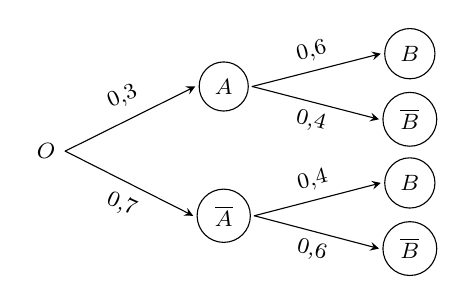
\begin{tikzpicture}[scale=0.8, font=\footnotesize, line join=round, line cap=round, >=stealth]
			\def\gocm{20}
			\def\gocn{10}
			\def\r{3}
			\tikzset{s/.style={outer sep=0.5 mm,draw=black,circle,minimum width=0.5cm,rounded corners=1mm}}
			\path(0,0)node(O){$O$}++(\gocm:\r)node[s](A1){$A$}++(\gocn:\r)node[s](A2){$B$};
			\path(A1)++({-\gocn}:\r)node[s](a2){$\overline{B}$};
			\path(O)++(-\gocm:\r)node[s](B1){$\overline{A}$}++(\gocn:\r)node[s](B2){$B$};
			\path(B1)++({-\gocn}:\r)node[s](b2){$\overline{B}$};
			\foreach \x/\y in {
				O/A1,A1/A2,
				O/B1,B1/B2,
				A1/a2,
				B1/b2}
			\draw[-stealth](\x.east)--(\y.west);
			\path(O)--(A1.west)node[pos=0.5,above,sloped]{$0{,}3$}(O)--(B1.west)node[pos=0.5,below,sloped]{$0{,}7$}(B1.east)--(B2.west)node[pos=0.5,above,sloped]{$0{,}4$}(A1.east)--(A2.west)node[pos=0.5,above,sloped]{$0{,}6$}
			(A1.east)--(a2.west)node[pos=0.5,below,sloped]{$0{,}4$}
			(B1.east)--(b2.west)node[pos=0.5,below,sloped]{$0{,}6$};
		\end{tikzpicture}
	}
	\loigiai{
		Áp dụng công thức xác suất toàn phần
		$$\mathrm{P}\left(B\right)=\mathrm{P}\left(A\right)\cdot\mathrm{P}\left(B\mid A\right)+\mathrm{P}\left(\overline{A}\right)\cdot\mathrm{P}\left(B\mid \overline{A}\right)=0{,}3\cdot 0{,}6+0{,}7\cdot 0{,}4=0{,}46.$$
	}	
\end{ex}
%%%=============================%%%

%%%=============EX_6=============%%%
\begin{ex}[28 chuyên đề - Nguyễn Bảo Vương]%[2D6H2-4]%[Dự án đề cương 3 khối NH24-25-Dot 1-Ngưng Trần]
	\immini{Cho sơ đồ hình cây dưới đây. Xác suất của biến cố $A$ khi biết biến cố $B$ đã xảy ra là
		\choice
		{$\dfrac{21}{23}$}
		{$\dfrac{14}{23}$}
		{$\dfrac{6}{23}$}
		{\True $\dfrac{9}{23}$}
	}{
		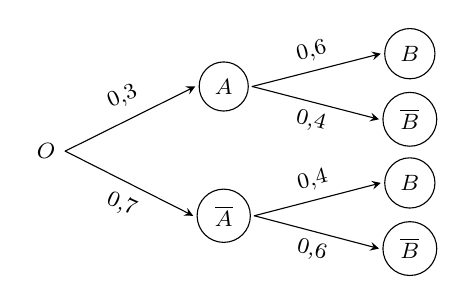
\begin{tikzpicture}[scale=0.8, font=\footnotesize, line join=round, line cap=round, >=stealth]
			\def\gocm{20}
			\def\gocn{10}
			\def\r{3}
			\tikzset{s/.style={outer sep=0.5 mm,draw=black,circle,minimum width=0.5cm,rounded corners=1mm}}
			\path(0,0)node(O){$O$}++(\gocm:\r)node[s](A1){$A$}++(\gocn:\r)node[s](A2){$B$};
			\path(A1)++({-\gocn}:\r)node[s](a2){$\overline{B}$};
			\path(O)++(-\gocm:\r)node[s](B1){$\overline{A}$}++(\gocn:\r)node[s](B2){$B$};
			\path(B1)++({-\gocn}:\r)node[s](b2){$\overline{B}$};
			\foreach \x/\y in {
				O/A1,A1/A2,
				O/B1,B1/B2,
				A1/a2,
				B1/b2}
			\draw[-stealth](\x.east)--(\y.west);
			\path(O)--(A1.west)node[pos=0.5,above,sloped]{$0{,}3$}(O)--(B1.west)node[pos=0.5,below,sloped]{$0{,}7$}(B1.east)--(B2.west)node[pos=0.5,above,sloped]{$0{,}4$}(A1.east)--(A2.west)node[pos=0.5,above,sloped]{$0{,}6$}
			(A1.east)--(a2.west)node[pos=0.5,below,sloped]{$0{,}4$}
			(B1.east)--(b2.west)node[pos=0.5,below,sloped]{$0{,}6$};
		\end{tikzpicture}
	}
	\loigiai{
		Áp dụng công thức Bayes, ta có
		$$\mathrm{P}\left(A\mid B\right)=\dfrac{\mathrm{P}\left(A\right)\cdot \mathrm{P}\left(B\mid A\right)}{\mathrm{P}\left(B\right)}$$
		Mặt khác theo công thức xác suất toàn phần, ta có
		$$\mathrm{P}\left(B\right)=\mathrm{P}\left(A\right)\cdot\mathrm{P}\left(B \mid A\right)+\mathrm{P}\left(\overline{A}\right)\cdot\mathrm{P}\left(B \mid\overline{A}\right)=0{,}3\cdot 0{,}6+0{,}7\cdot 0{,}4=0{,}18+0{,}28=0{,}46$$.
		Vậy 
		$\mathrm{P}\left(A\mid B\right)=\dfrac{0{,}3\cdot 0{,}6}{0{,}46}=\dfrac{0{,}18}{0{,}46}=\dfrac{9}{23}$.
		
	}
\end{ex}
%%%=============================%%%

%%%=============EX_7=============%%%
\begin{ex}[28 chuyên đề - Nguyễn Bảo Vương]%[2D6H2-4]%[Dự án đề cương 3 khối NH24-25-Dot 1-Ngưng Trần]
	\immini{Cho sơ đồ hình cây dưới đây. Xác suất của biến cố $A$ khi biết biến cố $\overline{B}$ đã xảy ra là
		\choice
		{$\dfrac{3}{9}$}
		{$\dfrac{3}{23}$}
		{$\dfrac{2}{23}$}
		{\True $\dfrac{2}{9}$}
	}{
		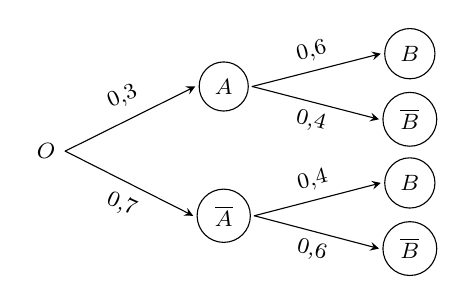
\begin{tikzpicture}[scale=0.8, font=\footnotesize, line join=round, line cap=round, >=stealth]
			\def\gocm{20}
			\def\gocn{10}
			\def\r{3}
			\tikzset{s/.style={outer sep=0.5 mm,draw=black,circle,minimum width=0.5cm,rounded corners=1mm}}
			\path(0,0)node(O){$O$}++(\gocm:\r)node[s](A1){$A$}++(\gocn:\r)node[s](A2){$B$};
			\path(A1)++({-\gocn}:\r)node[s](a2){$\overline{B}$};
			\path(O)++(-\gocm:\r)node[s](B1){$\overline{A}$}++(\gocn:\r)node[s](B2){$B$};
			\path(B1)++({-\gocn}:\r)node[s](b2){$\overline{B}$};
			\foreach \x/\y in {
				O/A1,A1/A2,
				O/B1,B1/B2,
				A1/a2,
				B1/b2}
			\draw[-stealth](\x.east)--(\y.west);
			\path(O)--(A1.west)node[pos=0.5,above,sloped]{$0{,}3$}(O)--(B1.west)node[pos=0.5,below,sloped]{$0{,}7$}(B1.east)--(B2.west)node[pos=0.5,above,sloped]{$0{,}4$}(A1.east)--(A2.west)node[pos=0.5,above,sloped]{$0{,}6$}
			(A1.east)--(a2.west)node[pos=0.5,below,sloped]{$0{,}4$}
			(B1.east)--(b2.west)node[pos=0.5,below,sloped]{$0{,}6$};
		\end{tikzpicture}
	}
	\loigiai{
		Áp dụng công thức Bayes, ta có
		$$\mathrm{P}\left(A\mid\overline{B}\right)=\dfrac{\mathrm{P}\left(A\right)\cdot \mathrm{P}\left(\overline{B}\mid A\right)}{\mathrm{P}\left(\overline{B}\right)}$$
		Mặt khác theo công thức xác suất toàn phần, ta có
		$$\mathrm{P}\left(\overline{B}\right)=\mathrm{P}\left(A\right)\cdot\mathrm{P}\left(\overline{B}\mid A\right)+\mathrm{P}\left(\overline{A}\right)\cdot\mathrm{P}\left(\overline{B}\mid\overline{A}\right)=0{,}3\cdot 0{,}4+0{,}7\cdot 0{,}6=0{,}12+0{,}42=0{,}54.$$
		Vậy 
		$\mathrm{P}\left(A\mid\overline{B}\right)=\dfrac{0{,}3\cdot 0{,}4}{0{,}54}=\dfrac{0{,}12}{0{,}54}=\dfrac{2}{9}$.
		
	}
\end{ex}
%%%=============================%%%

%%%=============EX_8=============%%%
\begin{ex}[28 chuyên đề - Nguyễn Bảo Vương]%[2D6N2-1]%[Dự án đề cương 3 khối NH24-25-Dot 1-Ngưng Trần]
	Cho các biến cố $A$ và $B$ sao cho $0<\mathrm{P}\left(A\right)<1$, $0<\mathrm{P}\left(B\right)<1$. Khẳng định nào sau đây là đúng?
	\choice
	{\True $\mathrm{P}\left(B\right)=\mathrm{P}\left(A\cap B\right)+\mathrm{P}\left(\overline{A}\cap B\right)$}
	{$\mathrm{P}\left(A\right)=\mathrm{P}\left(\overline{A}\cap\overline{B}\right)+\mathrm{P}\left(A\cap B\right)$}
	{$\mathrm{P}\left(B\right)=\mathrm{P}\left(\overline{A}\cap B\right)+\mathrm{P}\left(A\cap\overline{B}\right)$}
	{$\mathrm{P}\left(A\right)=\mathrm{P}\left(A\cap B\right)+\mathrm{P}\left(\overline{A}\cap B\right)$}
	\loigiai{
		Vì $(A\cap B)\cap\left(\overline{A}\cap B\right)=\left(A\cap\overline{A}\right)\cap B=\varnothing\cap B=\varnothing$ nên $A\cap B$ và $\overline{A}\cap B$ là hai biến cố là xung khắc.\\
		Ta có $\left(A\cap B\right)\cup\left(\overline{A}\cap B\right)=\left(A\cap\overline{A}\right)\cup B=\varnothing\cup B=B$.\\ 
		Do đó, $\mathrm{P}\left(B\right)=\mathrm{P}\left(A\cap B\right)+\mathrm{P}\left(\overline{A}\cap B\right)$.
	}
	
\end{ex}
%%%=============================%%%

%%%=============EX_9=============%%%
\begin{ex}[28 chuyên đề - Nguyễn Bảo Vương]%[2D6N2-1]%[Dự án đề cương 3 khối NH24-25-Dot 1-Ngưng Trần]
	Cho các biến cố $A$ và $B$ sao cho $0<\mathrm{P}\left(A\right)<1$, $0<\mathrm{P}\left(B\right)<1$, khẳng định nào sau đây là đúng?
	\choice
	{$\mathrm{P}\left(B\right)=\mathrm{P}\left(B\right)\cdot\mathrm{P}\left(A\mid B\right)+\mathrm{P}\left(\overline{B}\right)\cdot\mathrm{P}\left(A\mid\overline{B}\right)$}
	{\True $\mathrm{P}\left(A\right)=\mathrm{P}\left(B\right)\cdot\mathrm{P}\left(A\mid B\right)+\mathrm{P}\left(\overline{B}\right)\cdot\mathrm{P}\left(A\mid\overline{B}\right)$}
	{$\mathrm{P}\left(A\right)=\mathrm{P}\left(B\right)\cdot\mathrm{P}\left(B\mid A\right)+\mathrm{P}\left(\overline{B}\right)\cdot\mathrm{P}\left(A\mid B\right)$}
	{$\mathrm{P}\left(B\right)=\mathrm{P}\left(A\right)\cdot\mathrm{P}\left(B\mid A\right)+\mathrm{P}\left(\overline{B}\right)\cdot\mathrm{P}\left(A\mid B\right)$}
	\loigiai{
		Áp dụng công thức xác suất toàn phần, ta có
		$$\mathrm{P}\left(A\right)=\mathrm{P}\left(B\right)\cdot\mathrm{P}\left(A\mid B\right)+\mathrm{P}\left(\overline{B}\right)\cdot\mathrm{P}\left(A\mid\overline{B}\right)$$
	}
\end{ex}
%%%=============================%%%

%%%=============EX_10=============%%%
\begin{ex}[28 chuyên đề - Nguyễn Bảo Vương]%[2D6H2-2]%[Dự án đề cương 3 khối NH24-25-Dot 1-Ngưng Trần]
	\immini{Cho sơ đồ hình cây dưới đây. Xác suất để xảy ra biến cố $\overline{B}$ là
		\choice
		{$0{,}46$}
		{\True $0{,}54$}
		{$0{,}1$}
		{$0{,}4$}
	}{
		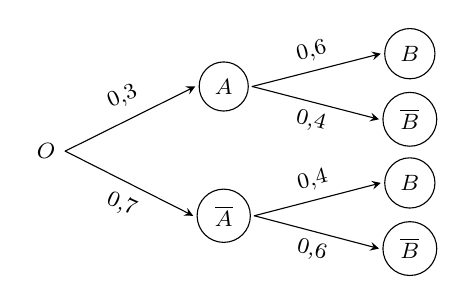
\begin{tikzpicture}[scale=0.8, font=\footnotesize, line join=round, line cap=round, >=stealth]
			\def\gocm{20}
			\def\gocn{10}
			\def\r{3}
			\tikzset{s/.style={outer sep=0.5 mm,draw=black,circle,minimum width=0.5cm,rounded corners=1mm}}
			\path(0,0)node(O){$O$}++(\gocm:\r)node[s](A1){$A$}++(\gocn:\r)node[s](A2){$B$};
			\path(A1)++({-\gocn}:\r)node[s](a2){$\overline{B}$};
			\path(O)++(-\gocm:\r)node[s](B1){$\overline{A}$}++(\gocn:\r)node[s](B2){$B$};
			\path(B1)++({-\gocn}:\r)node[s](b2){$\overline{B}$};
			\foreach \x/\y in {
				O/A1,A1/A2,
				O/B1,B1/B2,
				A1/a2,
				B1/b2}
			\draw[-stealth](\x.east)--(\y.west);
			\path(O)--(A1.west)node[pos=0.5,above,sloped]{$0{,}3$}(O)--(B1.west)node[pos=0.5,below,sloped]{$0{,}7$}(B1.east)--(B2.west)node[pos=0.5,above,sloped]{$0{,}4$}(A1.east)--(A2.west)node[pos=0.5,above,sloped]{$0{,}6$}
			(A1.east)--(a2.west)node[pos=0.5,below,sloped]{$0{,}4$}
			(B1.east)--(b2.west)node[pos=0.5,below,sloped]{$0{,}6$};
		\end{tikzpicture}
	}
	\loigiai{
		Áp dụng công thức xác suất toàn phần
		$$\mathrm{P}\left(\overline{B}\right)=\mathrm{P}\left(A\right)\cdot\mathrm{P}\left(\overline{B}\mid A\right)+\mathrm{P}\left(\overline{A}\right)\cdot\mathrm{P}\left(\overline{B}\mid \overline{A}\right)=0{,}3\cdot 0{,}4+0{,}7\cdot 0{,}6=0{,}54.$$
	}	
\end{ex}
%%%=============================%%%

%%%=============EX_11=============%%%
\begin{ex}[28 chuyên đề - Nguyễn Bảo Vương]%[2D6N2-2]%[Dự án đề cương 3 khối NH24-25-Dot 1-Ngưng Trần]
	Cho các biến cố $A$, $B$ thỏa mãn $\mathrm{P}\left(A\cap B\right)=\dfrac{1}{3}$, $\mathrm{P}\left(\overline{A}\cap B\right)=\dfrac{1}{4}$. Xác suất để biến cố $B$ xảy ra là
	\choice
	{$\mathrm{P}\left(B\right)=\dfrac{1}{12}$}
	{$\mathrm{P}\left(B\right)=\dfrac{5}{12}$}
	{$\mathrm{P}\left(B\right)=\dfrac{3}{4}$}
	{\True $\mathrm{P}\left(B\right)=\dfrac{7}{12}$}
	\loigiai{
		Ta có $\mathrm{P}\left(B\right)=\mathrm{P}\left(A\cap B\right)+\mathrm{P}\left(\overline{A}\cap B\right)=\dfrac{1}{3}+\dfrac{1}{4}=\dfrac{7}{12}$.
	}
\end{ex}
%%%=============================%%%

%%%=============EX_12=============%%%
\begin{ex}[28 chuyên đề - Nguyễn Bảo Vương]%[2D6H2-2]%[Dự án đề cương 3 khối NH24-25-Dot 1-Ngưng Trần]
	Cho các biến cố $A$, $B$ với $\mathrm{P}\left(B\right)=0{,}35$, $\mathrm{P}\left(A\mid B\right)=0{,}75$, $\mathrm{P}\left(A\mid\overline{B}\right)=0{,}12$. Xác suất để biến cố $A$ xảy ra là
	\choice
	{$\mathrm{P}\left(A\right)=0{,}36$}
	{\True $\mathrm{P}\left(A\right)=0{,}3405$}
	{$\mathrm{P}\left(A\right)=0{,}4242$}
	{$\mathrm{P}\left(A\right)=0{,}24$}
	\loigiai{
		Ta có $\mathrm{P}\left(\overline{B}\right)=1-\mathrm{P}\left(B\right)=1-0{,}35=0{,}65$.\\
		Áp dụng công thức xác suất toàn phần, ta có
		$$\mathrm{P}\left(A\right)=\mathrm{P}\left(B\right)\cdot\mathrm{P}\left(A\mid B\right)+\mathrm{P}\left(\overline{B}\right)\cdot\mathrm{P}\left(A\mid\overline{B}\right)
		=0{,}35\cdot0{,}75+0{,}65\cdot0{,}12=0{,}2625+0{,}078=0{,}3405.$$
	}
\end{ex}
%%%=============================%%%

%%%=============EX_13=============%%%
\begin{ex}[28 chuyên đề - Nguyễn Bảo Vương]%[2D6N2-3]%[Dự án đề cương 3 khối NH24-25-Dot 1-Ngưng Trần]
	Cho hai biến cố ngẫu nhiên $A$ và $B$ có $\mathrm{P}\left(B\right)=0{,}5$, $\mathrm{P}\left(A\mid B\right)=0{,}24$, $\mathrm{P}\left(A\mid\overline{B}\right)=0{,}16$. Khi đó, $\mathrm{P}\left(B\mid A\right)$ bằng
	\choice
	{$0{,}3$}
	{$0{,}5$}
	{$0{,}4$}
	{\True $0{,}6$}
	\loigiai{
		Áp dụng công thức Bayes, ta có
		$$\mathrm{P}\left(B\mid A\right)=\dfrac{\mathrm{P}\left(B\right)\cdot\mathrm{P}\left(A\mid B\right)}{\mathrm{P}\left(B\right)\cdot\mathrm{P}\left(A\mid B\right)+\mathrm{P}\left(\overline{B}\right)\cdot\mathrm{P}\left(A\mid\overline{B}\right)}=\dfrac{0{,}5\cdot0{,}24}{0{,}5\cdot0{,}24+0{,}5\cdot0{,}16}=0{,}6.$$
	}
\end{ex}
%%%=============================%%%

%%%=============EX_14=============%%%
\begin{ex}[28 chuyên đề - Nguyễn Bảo Vương]%[2D6H2-3]%[Dự án đề cương 3 khối NH24-25-Dot 1-Ngưng Trần]
	Trong một kì sát hạch lái xe có $65\%$ thí sinh là nam. Biết rằng có $80\%$ thí sinh nam và $70\%$ thí sinh nữ đỗ kì sát hạch này. Gọi các biến cố $A\colon$ \lq\lq Thí sinh tham gia sát hạch là nam\rq\rq, $B\colon$ \lq\lq Thí sinh đỗ kì sát hạch\rq\rq. Giá trị biểu thức 
	$\dfrac{\mathrm{P}\left(B\right)\cdot\mathrm{P}\left(A\mid B\right)}{\mathrm{P}\left(B\right)\cdot\mathrm{P}\left(A\mid B\right)+\mathrm{P}\left(\overline{B}\right)\cdot\mathrm{P}\left(A\mid\overline{B}\right)}$ bằng với
	\choice
	{$0{,}6$}
	{$0{,}72$}
	{\True $0{,}8$}
	{$0{,}76$}
	\loigiai{
		Ta có
		$$\dfrac{\mathrm{P}\left(B\right)\cdot\mathrm{P}\left(A\mid B\right)}{\mathrm{P}\left(B\right)\cdot\mathrm{P}\left(A\mid B\right)+\mathrm{P}\left(\overline{B}\right)\cdot\mathrm{P}\left(A\mid\overline{B}\right)}=\dfrac{\mathrm{P}\left(A\cap B\right)}{\mathrm{P}\left(A\right)}=\mathrm{P}\left(B\mid A\right)=0{,}8.$$
	}
\end{ex}
%%%=============================%%%

%%%=============EX_15=============%%%
\begin{ex}[28 chuyên đề - Nguyễn Bảo Vương]%[2D6N2-1]%[Dự án đề cương 3 khối NH24-25-Dot 1-Ngưng Trần]
	Cho các biến cố $A$ và $B$ sao cho $0<\mathrm{P}\left(A\right)<1$, $0<\mathrm{P}\left(B\right)<1$. Khẳng định nào sau đây là đúng?
	\choice
	{\True $\mathrm{P}\left(B\mid A\right)=\dfrac{\mathrm{P}\left(B\right)\cdot\mathrm{P}\left(A\mid B\right)}{\mathrm{P}\left(B\right)\cdot\mathrm{P}\left(A\mid B\right)+\mathrm{P}\left(\overline{B}\right)\cdot\mathrm{P}\left(A\mid\overline{B}\right)}$}
	{$\mathrm{P}\left(A\mid B\right)=\dfrac{\mathrm{P}\left(B\right)\cdot\mathrm{P}\left(A\mid B\right)}{\mathrm{P}\left(A\right)}$}
	{$\mathrm{P}\left(B\mid A\right)=\dfrac{\mathrm{P}\left(A\cap B\right)\cdot\mathrm{P}\left(A\mid B\right)}{\mathrm{P}\left(B\right)\cdot\mathrm{P}\left(A\mid B\right)+\mathrm{P}\left(\overline{B}\right)\cdot\mathrm{P}\left(A\mid\overline{B}\right)}$}
	{$\mathrm{P}\left(A\mid B\right)=\dfrac{\mathrm{P}\left(B\mid A\right)}{\mathrm{P}\left(B\right)}$}
	\loigiai{
		Ta có $\mathrm{P}\left(B\mid A\right)=\dfrac{\mathrm{P}\left(B\right)\cdot\mathrm{P}\left(A\mid B\right)}{\mathrm{P}\left(B\right)\cdot\mathrm{P}\left(A\mid B\right)+\mathrm{P}\left(\overline{B}\right)\cdot\mathrm{P}\left(A\mid\overline{B}\right)}$.
	}
\end{ex}
%%%=============================%%%

%%%=============EX_16=============%%%
\begin{ex}[28 chuyên đề - Nguyễn Bảo Vương]%[2D6H2-2]%[Dự án đề cương 3 khối NH24-25-Dot 1-Ngưng Trần]
	Cho các biến cố $A$, $B$ thỏa mãn $\mathrm{P}\left(\overline{A}\cap B\right)=0{,}35$, $\mathrm{P}\left(A\right)=0{,}25$, $\mathrm{P}\left(B\right)=0{,}6$. Giá trị $\mathrm{P}\left(A\mid B\right)$ bằng:
	\choice
	{$\dfrac{3}{5}$}
	{$\dfrac{2}{5}$}
	{\True $\dfrac{1}{3}$}
	{$\dfrac{2}{3}$}
	\loigiai{
		Ta có
		$$\mathrm{P}\left(\overline{A}\right)=1-\mathrm{P}\left(A\right)=0{,}75
		\Rightarrow \mathrm{P}\left(\overline{A}\cap B\right)=\mathrm{P}\left(\overline{A}\right)-\mathrm{P}\left(\overline{A}\cap B\right)=0{,}75-0{,}35=0{,}4.$$
		Suy ra
		$$\mathrm{P}\left(\overline{A}\mid B\right)=\dfrac{\mathrm{P}\left(\overline{A}\cap B\right)}{\mathrm{P}\left(B\right)}=\dfrac{0{,}4}{0{,}6}=\dfrac{2}{3}
		\Rightarrow \mathrm{P}\left(A\mid B\right)=1-\dfrac{2}{3}=\dfrac{1}{3}.$$
		
	}
\end{ex}
%%%=============================%%%

%%%=============EX_17=============%%%
\begin{ex}[28 chuyên đề - Nguyễn Bảo Vương]%[2D6N2-1]%[Dự án đề cương 3 khối NH24-25-Dot 1-Ngưng Trần]
	Cho $A$, $B$ là các biến cố của một phép thử $T$. Biết rằng $\mathrm{P}\left(A\right)>0$ và $0<\mathrm{P}\left(B\right)<1$. Xác suất của biến cố $B$ với điều kiện biến cố $A$ đã xảy ra được tính theo công thức nào sau đây?
	\choice
	{$\mathrm{P}\left(B\mid A\right)=\dfrac{\mathrm{P}\left(A\right)\cdot\mathrm{P}\left(A\mid B\right)}{\mathrm{P}\left(B\right)\cdot\mathrm{P}\left(A\mid B\right)+\mathrm{P}\left(\overline{B}\right)\cdot\mathrm{P}\left(A\mid\overline{B}\right)}$}
	{\True $\mathrm{P}\left(B\mid A\right)=\dfrac{\mathrm{P}\left(B\right)\cdot\mathrm{P}\left(A\mid B\right)}{\mathrm{P}\left(B\right)\cdot\mathrm{P}\left(A\mid B\right)+\mathrm{P}\left(\overline{B}\right)\cdot\mathrm{P}\left(A\mid\overline{B}\right)}$}
	{$\mathrm{P}\left(B\mid A\right)=\dfrac{\mathrm{P}\left(B\right)\cdot\mathrm{P}\left(A\mid B\right)}{\mathrm{P}\left(B\right)\cdot\mathrm{P}\left(\overline{A}\mid B\right)+\mathrm{P}\left(\overline{B}\right)\cdot\mathrm{P}\left(A\mid\overline{B}\right)}$}
	{$\mathrm{P}\left(B\mid A\right)=\dfrac{\mathrm{P}\left(A\right)\cdot\mathrm{P}\left(A\mid B\right)}{\mathrm{P}\left(A\right)\cdot\mathrm{P}\left(\overline{B}\right)\cdot\mathrm{P}\left(A\mid\overline{B}\right)}$}
	\loigiai{
		Theo công thức Bayes, ta có
		$$\mathrm{P}\left(B\mid A\right)=\dfrac{\mathrm{P}\left(B\right)\cdot\mathrm{P}\left(A\mid B\right)}{\mathrm{P}\left(B\right)\cdot\mathrm{P}\left(A\mid B\right)+\mathrm{P}\left(\overline{B}\right)\cdot\mathrm{P}\left(A\mid\overline{B}\right)}.$$
	}
\end{ex}
%%%=============================%%%

%%%=============EX_18=============%%%
\begin{ex}[28 chuyên đề - Nguyễn Bảo Vương]%[2D6N2-3]%[Dự án đề cương 3 khối NH24-25-Dot 1-Ngưng Trần]
	Nếu hai biến cố $A$, $B$ thỏa mãn $\mathrm{P}\left(A\right)=0{,}3$, $\mathrm{P}\left(B\right)=0{,}6$ và $\mathrm{P}\left(A\mid B\right)=0{,}4$ thì $\mathrm{P}\left(B\mid A\right)$ bằng
	\choice
	{$0{,}5$}
	{$0{,}6$}
	{\True $0{,}8$}
	{$0{,}2$}
	\loigiai{
		Theo công thức Bayes, ta có
		$$\mathrm{P}\left(B\mid A\right)=\dfrac{\mathrm{P}\left(B\right)\cdot\mathrm{P}\left(A\mid B\right)}{\mathrm{P}\left(A\right)}=\dfrac{0{,}6\cdot0{,}4}{0{,}3}=0{,}8.$$
	}
\end{ex}
%%%=============================%%%

%%%=============EX_19=============%%%
\begin{ex}[28 chuyên đề - Nguyễn Bảo Vương]%[2D6H2-2]%[Dự án đề cương 3 khối NH24-25-Dot 1-Ngưng Trần]
	\immini{
		Một học sinh đi học muộn với xác suất là $0{,}3$. Nếu người đó đi học muộn thì xác suất để người đó ăn sáng là $0{,}2$. Nếu người đó không đi học muộn thì xác suất để người đó ăn sáng là $0{,}6$. Xác suất của biến cố người đó không ăn sáng là
		\choice
		{$0{,}48$}
		{$0{,}8$}
		{\True $0{,}52$}
		{$0{,}9$}
	}{
%		\begin{center}
			\begin{tikzpicture}[scale=0.8, font=\footnotesize, line join=round, line cap=round, >=stealth]
			\def\gocm{20}
			\def\gocn{10}
			\def\r{5}
			\tikzset{s/.style={outer sep=0.5 mm,draw=black,rectangle,minimum width=2cm,rounded corners=1mm}}
			\path(0,0)node(O){$O$}++(\gocm:\r)node[s](A1){$\text{Đi học muộn}$}++(\gocn:\r)node[s](A2){$\text{Ăn sáng}$};
			\path(A1)++({-\gocn}:\r)node[s](a2){$\text{Không ăn sáng}$};
			\path(O)++(-\gocm:\r)node[s](B1){$\text{Không đi học muộn}$}++(\gocn:\r)node[s](B2){$\text{Ăn sáng}$};
			\path(B1)++({-\gocn}:\r)node[s](b2){$\text{Không ăn sáng}$};
			\foreach \x/\y in {
				O/A1,A1/A2,
				O/B1,B1/B2,
				A1/a2,
				B1/b2}
			\draw[-stealth](\x.east)--(\y.west);
			\path(O)--(A1.west)node[pos=0.5,above,sloped]{$0{,}3$}(O)--(B1.west)node[pos=0.5,below,sloped]{$0{,}7$}(B1.east)--(B2.west)node[pos=0.5,above,sloped]{$0{,}6$}(A1.east)--(A2.west)node[pos=0.5,above,sloped]{$0{,}2$}
			(A1.east)--(a2.west)node[pos=0.5,below,sloped]{$0{,}8$}
			(B1.east)--(b2.west)node[pos=0.5,below,sloped]{$0{,}4$};
		\end{tikzpicture}
%		\end{center}
	}
	\loigiai{
		Áp dụng công thức xác suất toàn phần, ta có xác suất của biến cố người đó không ăn sáng là $0{,}3\cdot0{,}8+0{,}7\cdot0{,}4=0{,}52$.
		
	}	
\end{ex}
%%%=============================%%%

%%%=============EX_20=============%%%
\begin{ex}[28 chuyên đề - Nguyễn Bảo Vương]%[2D6H2-2]%[Dự án đề cương 3 khối NH24-25-Dot 1-Ngưng Trần]
	\immini{Một học sinh đi học muộn với xác suất là $0{,}3$. Nếu người đó đi học muộn thì xác suất để người đó ăn sáng là $0{,}2$. Nếu người đó không đi học muộn thì xác suất để người đó ăn sáng là $0{,}6$. Xác suất của biến cố người đó ăn sáng là
		\choice
		{\True $0{,}48$}
		{$0{,}8$}
		{$0{,}52$}
		{$0{,}9$}
	}{
		\begin{tikzpicture}[scale=0.8, font=\footnotesize, line join=round, line cap=round, >=stealth]
			\def\gocm{20}
			\def\gocn{10}
			\def\r{5}
			\tikzset{s/.style={outer sep=0.5 mm,draw=black,rectangle,minimum width=2cm,rounded corners=1mm}}
			\path(0,0)node(O){$O$}++(\gocm:\r)node[s](A1){$\text{Đi học muộn}$}++(\gocn:\r)node[s](A2){$\text{Ăn sáng}$};
			\path(A1)++({-\gocn}:\r)node[s](a2){$\text{Không ăn sáng}$};
			\path(O)++(-\gocm:\r)node[s](B1){$\text{Không đi học muộn}$}++(\gocn:\r)node[s](B2){$\text{Ăn sáng}$};
			\path(B1)++({-\gocn}:\r)node[s](b2){$\text{Không ăn sáng}$};
			\foreach \x/\y in {
				O/A1,A1/A2,
				O/B1,B1/B2,
				A1/a2,
				B1/b2}
			\draw[-stealth](\x.east)--(\y.west);
			\path(O)--(A1.west)node[pos=0.5,above,sloped]{$0{,}3$}(O)--(B1.west)node[pos=0.5,below,sloped]{$0{,}7$}(B1.east)--(B2.west)node[pos=0.5,above,sloped]{$0{,}6$}(A1.east)--(A2.west)node[pos=0.5,above,sloped]{$0{,}2$}
			(A1.east)--(a2.west)node[pos=0.5,below,sloped]{$0{,}8$}
			(B1.east)--(b2.west)node[pos=0.5,below,sloped]{$0{,}4$};
		\end{tikzpicture}
	}
	\loigiai{
		Áp dụng công thức xác suất toàn phần, ta có xác suất của biến cố người đó ăn sáng là $0{,}3\cdot0{,}2+0{,}7\cdot0{,}6=0{,}48$.
		
	}	
\end{ex}
%%%=============================%%%
\Closesolutionfile{ans}

\ind{PHẦN II.} \inden{Câu trắc nghiệm đúng sai. Trong mỗi ý a), b), c), d) ở mỗi câu, học sinh chọn đúng hoặc sai.}\\
\setcounter{ex}{0}
\Opensolutionfile{ans}[ans/2D2-Bai2-DS]%--Đặt tên 2D2-Bai2-DS

%%%=========TF_1=========%%%
\begin{ex}[Trích đề thi thử - THPT Trần Nguyên Hãn - Hải Phòng - Năm học: 2024-2025]%[2D6H2-4]%[Dự án đề cương 3 khối NH24-25-Dot 1-Ngưng Trần]
	Trước khi đưa một loại sản phẩm ra thị trường, người ta đā phỏng vấn ngẫu nhiên 200 khách hàng về sản phẩm đó. Kết quả thống kê có 105 người trả lời \lq\lq sẽ mua\rq\rq; có 95 người trả lời \lq\lq không mua\rq\rq. Kinh nghiệm cho thấy tỉ lệ khách hàng thực sự sẽ mua sản phẩm tương ứng với những cách trả lời \lq\lq sē mua\rq\rq~và~\lq\lq không mua\rq\rq~ lần lượt là $70 \%$ và $30 \%$. Gọi $A$ là biến cố \lq\lq Người được phỏng vấn thực sự sē mua sản phẩm\rq\rq. Gọi $B$ là biến cố \lq\lq Người được phỏng vấn trả lời sē mua sản phẩm\rq\rq.
	\choiceTFt
	{\True Xác suất $\mathrm{P}\left(B\right)=\dfrac{21}{40}$ và $\mathrm{P}\left(\overline{B}\right)=\dfrac{19}{40}$}
	{Xác suất có điều kiện $\mathrm{P}\left(A\mid B\right)=0{,}3$}
	{\True Xác suất $\mathrm{P}\left(A\right)=0{,}51$}
	{Trong số những người được phỏng vấn thực sự sẽ mua sản phẩm có $70\%$ người đã trả lời "sẽ mua" khi được phỏng vấn (kết quả tính theo phần trăm được làm tròn đến hàng đơn vị)}
	\loigiai{
		\begin{itemchoice}
			\itemch Xác suất $\mathrm{P}\left(B\right)=\dfrac{105}{200}=\dfrac{21}{40}$; $\mathrm{P}\left(\overline{B}\right)=1-\mathrm{P}\left(B\right)=\dfrac{19}{40}$.
			\itemch Theo đề bài: Kinh nghiệm cho thấy tỉ lệ khách hàng thực sự sẽ mua sản phẩm tương ứng với những cách trả lời \lq\lq ~sẽ mua\rq\rq~ là $70\%$.\\
			Do đó xác suất có điều kiện $\mathrm{P}\left(A\mid B\right)=0{,}7$.
			\itemch Áp dụng công thức xác suất toàn phần, ta có
			$$\mathrm{P}\left(A\right)=\mathrm{P}\left(A\mid B\right)\cdot\mathrm{P}\left(B\right)+\mathrm{P}\left(A\mid \overline{B}\right)\cdot\mathrm{P}\left(\overline{B}\right)=0{,}7\cdot\dfrac{21}{40}+0{,}3\cdot\dfrac{19}{40}=0{,}51.$$
			\itemch Áp dụng công thức Bayes, ta có
			$$\mathrm{P}\left(B\mid A\right)=\dfrac{\mathrm{P}\left(A\mid B\right)\cdot\mathrm{P}\left(B\right)}{\mathrm{P}(A)}=\dfrac{0{,}7\cdot\dfrac{21}{40}}{0{,}51}\approx 0{,}72.$$
		\end{itemchoice}
	}
\end{ex}

%%%=========TF_2=========%%%
\begin{ex}[Trích đề thi thử - Bình Thuận - Năm học: 2024-2025]%[2D6H2-4]%[Dự án đề cương 3 khối NH24-25-Dot 1-Ngưng Trần]
	Một nghiên cứu đã chỉ ra rằng tỉ lệ người lao phổi trong nhóm $X$ những người mắc phải hội chứng suy giảm miễn dịch $H$ là $15{,}2 \%$. Kết quả nghiên cứu về một số triệu chứng lâm sàng như có ho trong vòng bốn tuần, hoặc có bị sốt trong vòng bốn tuần, hoặc ra mồ hôi ban đêm từ ba tuần trở lên của nhóm $X$ cho thấy trong số những người mắc bệnh lao phổi, có $93{,}2 \%$ trường hợp có ít nhất một triệu chứng; trong số những người không mắc bệnh lao phổi, có $35{,}8 \%$ trường hợp không có triệu chứng nào.
	\choiceTFt
	{\True Gặp ngẫu nhiên một bệnh nhân thuộc nhóm $X$, xác suất bệnh nhân bị lao phổi là $0{,}152$}
	{Gặp được bệnh nhân không mắc bệnh lao phổi, xác suất bệnh nhân đó có ít nhất một triệu chứng trên là $0{,}358$}
	{Có $70 \%$ bệnh nhân thuộc nhóm $X$ có ít nhất một triệu chứng trên (kết quả tính theo phần trăm được làm tròn đến hàng đơn vị)}
	{\True Trong số những bệnh nhân có ít nhất một triệu chứng trên, có $21 \%$ người mắc bệnh lao phổi (kết quả tính theo phần trăm được làm tròn đến hàng đơn vị)}
	
	\loigiai{
		Gọi các biến cố\\
		$A$ là biến cố \lq\lq gặp được người bị lao phổi\rq\rq.\\
		$B$ là biến cố \lq\lq gặp được người có ít nhất một triệu chứng trong các triệu chứng trên\rq\rq.
		\begin{itemchoice}
			\itemch Xác suất bệnh nhân bị lao phổi là $\mathrm{P}\left(A\right)=0{,}152$.
			\itemch Ta có $\mathrm{P}\left(B\mid\overline{A}\right)=1-\mathrm{P}\left(\overline{B}\mid\overline{A}\right)=1-0{,}358=0{,}642$.
			\itemch Theo công thức xác suất toàn phần, ta có
			$$\mathrm{P}\left(B\right)=\mathrm{P}\left(B\mid A\right)\cdot\mathrm{P}\left(A\right)+\mathrm{P}\left(B\mid\overline{A}\right)\cdot\mathrm{P}\left(\overline{A}\right)=0{,}932\cdot 0{,}152+0{,}642\cdot 0{,}848=0{,}68608\approx 0{,}69.$$
			Vậy có $69\%$ bệnh nhân thuộc nhóm $X$ có ít nhất một triệu chứng trên.
			\itemch Theo công thức Bayes, ta có
			$$\mathrm{P}\left(A\mid B\right)=\dfrac{\mathrm{P}\left(B\mid A\right)\cdot\mathrm{P}\left(A\right)}{\mathrm{P}\left(B\right)}=\dfrac{0{,}932\cdot 0{,}152}{0{,}68608}\approx 0{,}21.$$
			Suy ra trong số những bệnh nhân có ít nhất một triệu chứng trên, có $21\%$ người mắc bệnh lao phổi.
		\end{itemchoice}
	}
\end{ex}

%%%=========TF_3=========%%%
\begin{ex}[Trích đề thi thử - THPT Lê Thánh Tông - Nguyễn Khuyến - Năm học: 2024-2025]%[2D6C2-4]%[Dự án đề cương 3 khối NH24-25-Dot 1-Ngưng Trần]
	Một túi chứa ba đồng xu công bằng (fair coin - tức đồng xu có đủ hai mặt sấp ngửa) và một đồng xu có hai mặt ngửa (double-headed coin). Một đồng xu được chọn ngẫu nhiên từ túi và được gieo để xem mặt hiện ra là ngửa hay sấp.
	\choiceTFt
	{Xác suất để đồng xu fair coin được chọn và mặt sấp xuất hiện bằng $\dfrac{1}{2}$}
	{\True Xác suất xuất hiện mặt ngửa bằng $\dfrac{5}{8}$}
	{Nếu biết mặt ngửa đã xuất hiện, xác suất đồng xu có hai mặt ngửa đã được chọn bằng $\dfrac{3}{5}$}
	{\True Nếu gieo đồng xu lần đầu xuất hiện mặt ngửa, xác suất để khi gieo đồng xu đó lần thứ hai vẫn xuất hiện mặt ngửa bằng $\dfrac{7}{10}$}
	
	\loigiai{
		
		\begin{itemchoice}
			\itemch Gọi biến cố $A\colon$ \lq\lq Chọn được một đồng xu fair coin\rq\rq\.\\
			Suy ra $\mathrm{P}\left(A\right)=\dfrac{3}{4}$; $ \mathrm{P}\left(\overline{A}\right)=\dfrac{1}{4}$.\\ 
			Gọi biến cố $B\colon$ \lq\lq Gieo đồng xu xuất hiện mặt sấp\rq\rq\.\\ Suy ra $\mathrm{P}\left(B\mid A\right)=\dfrac{1}{2}$; $\mathrm{P}\left(B\mid\overline{A}\right)=0$.\\ 
			Xác suất để đồng xu fair coin được chọn và mặt sấp xuất hiện bằng  
			$$\mathrm{P}\left(AB\right)=\mathrm{P}\left(A\right)\cdot\mathrm{P}\left(B\mid A\right)=\dfrac{3}{4}\cdot\dfrac{1}{2}=\dfrac{3}{8}.$$
			\itemch Ta có $\mathrm{P}\left(\overline{B}\mid A\right)=\dfrac{1}{2}$;  $\mathrm{P}\left(\overline{B}\mid \overline{A}\right)=1$.\\  
			Theo công thức xác suất toàn phần, ta có  
			$$\mathrm{P}\left(\overline{B}\right)=\mathrm{P}\left(A\right)\cdot\mathrm{P}\left(\overline{B}\mid A\right)+\mathrm{P}\left(\overline{A}\right)\cdot\mathrm{P}\left(\overline{B}\mid\overline{A}\right)=\dfrac{3}{4}\cdot\dfrac{1}{2}+\dfrac{1}{4}\cdot1=\dfrac{5}{8}.$$
			\itemch Nếu biết mặt ngửa đã xuất hiện, xác suất đồng xu có hai mặt ngửa đã được chọn chính là xác suất có điều kiện $\mathrm{P}\left(\overline{A}\mid \overline{B}\right)$. Theo công thức Bayes, ta có
			$$\mathrm{P}\left(\overline{A}\mid \overline{B}\right)=\dfrac{\mathrm{P}\left(\overline{A}\right)\cdot\mathrm{P}\left(\overline{B}\mid\overline{A}\right)}{\mathrm{P}\left(\overline{B}\right)}=\dfrac{\dfrac{1}{4}\cdot1}{\dfrac{5}{8}}=\dfrac{2}{5}.$$
			\itemch Gọi biến cố $E\colon$ \lq\lq Lần tung đầu tiên xuất hiện mặt ngửa\rq\rq\ và biến cố $F\colon$ \lq\lq Lần tung thứ hai xuất hiện mặt ngửa\rq\rq.  
			Ta có $\mathrm{P}\left(E\right)=\dfrac{3}{4}\cdot\dfrac{1}{2}+\dfrac{1}{4}\cdot1=\dfrac{5}{8}$. Ta tính $\mathrm{P}\left(E\cap F\right)$.
			\begin{itemize}
				\item Trường hợp 1: Chọn được đồng xu fair coin và mặt ngửa xuất hiện ở lần tung đầu tiên, xác suất lần tung thứ hai xuất hiện mặt ngửa là $\frac{1}{2}$ nên xác suất cả hai lần tung xuất hiện mặt ngửa từ các đồng xu fair coin bằng $\mathrm{P}\left(E\cap F\right)=\dfrac{3}{4}\cdot\dfrac{1}{2}\cdot\dfrac{1}{2}=\dfrac{3}{16}$.
				\item Trường hợp 2: Chọn được đồng xu double-headed coin thì xác xuất cả hai lần tung xuất hiện mặt ngửa bằng $\mathrm{P}\left(E\cap F\right)=\dfrac{1}{4}$.
			\end{itemize}
			Suy ra $\mathrm{P}\left(E\cap F\right)=\dfrac{3}{16}+\dfrac{4}{16}=\dfrac{7}{16}$.\\
			Vậy $\mathrm{P}\left(F\mid E\right)=\dfrac{\mathrm{P}\left(E\cap F\right)}{\mathrm{P}\left(E\right)}=\dfrac{7}{10}$.
		\end{itemchoice}
	}
\end{ex}

%%%=========TF_4=========%%%
\begin{ex}[Trích đề thi thử - THPT Nguyễn Khuyến - Lê Thánh Tông  - Năm học: 2024-2025]%[2D6V2-4]%[Dự án đề cương 3 khối NH24-25-Dot 1-Ngưng Trần]
	Xác suất để công ty $X$ thuê một trong hai công ty vệ tinh $A$ và $B$ tư vấn lần lượt là $0{,}4$ và $0{,}6$ . Theo kinh nghiệm khả năng $X$ phát sinh thêm chi phí khi sử dụng dịch vụ tư vấn của công ty $A$ và $B$ lần lượt là $0{,}05$ và $0{,}03$.
	\choiceTFt
	{\True Xác suất để $X$ có phát sinh thêm chi phí khi sử dụng dịch vụ tư vấn là $0{,}038$}
	{Biết $X$ có phát sinh thêm chi phí khi sử dụng dịch vụ tư vấn. Xác suất để $X$ thuê công ty $A$ tư vấn là $0{,}4737$}
	{Biết $X$ có phát sinh thêm chi phí khi sử dụng dịch vụ tư vấn. Xác suất để $X$ thuê công ty $B$ tư vấn là $0{,}5263$}
	{\True Biết $X$ không phát sinh thêm chi phí khi sử dụng dịch vụ tư vấn. Xác suất để $X$ thuê công ty $A$ tư vấn là $0{,}395$}
	
	\loigiai{
		
		\begin{itemchoice}
			\itemch Xét các biến cố:
			$M\colon$\lq\lq Công ty $X$ thuê công ty vệ tinh A tư vấn\rq\rq;\\
			$N\colon$\lq\lq Công ty $X$ có phát sinh thêm chi phí khi sử dụng dịch vụ tư vấn\rq\rq.\\
			Ta có $0,4+0,6=1$, do đó $\overline{M}$ là biến cố \lq\lq Công ty $X$ thuê công ty vệ tinh $B$ tư vấn\rq\rq.\\
			Theo đề bài ta được $\mathrm{P}\left(M\right)=0{,}4$; $\mathrm{P}\left(\overline{M}\right)=0{,}6$; $\mathrm{P}\left(N\mid M\right)=0{,}05$; $\mathrm{P}\left(N\mid\overline{M}\right)=0{,}03$.\\
			Áp dụng công thức xác suất toàn phần, ta có $$\mathrm{P}\left(N\right)=\mathrm{P}\left(M\right)\cdot\mathrm{P}\left(N\mid M\right)+\mathrm{P}\left(\overline{M}\right)\cdot\mathrm{P}\left(N\mid\overline{M}\right)
			=0{,}4\cdot0{,}05+0{,}6\cdot0{,}03=0{,}038.$$
			Suy ra xác suất để X có phát sinh thêm chi phí khi sử dụng dịch vụ tư vấn là $0{,}038$.\\
			\itemch Theo công thức Bayes, ta có
			$$\mathrm{P}(M\mid N)=\dfrac{\mathrm{P}(M)\cdot\mathrm{P}(N\mid M)}{\mathrm{P}(N)}=\dfrac{0{,}4\cdot0{,}05}{0{,}038}\approx0{,}5263.$$
			Vậy khi biết $X$ có phát sinh thêm chi phí thì xác suất để $X$ thuê công ty $A$ tư vấn là khoảng $0{,}5263$.
			\itemch Tương tự
			$$\mathrm{P}(\overline{M}\mid N)=\dfrac{\mathrm{P}(\overline{M})\cdot\mathrm{P}(N\mid\overline{M})}{\mathrm{P}(N)}=\dfrac{0{,}6\cdot0{,}03}{0{,}038}\approx0{,}4737.$$
			Vậy khi biết $X$ có phát sinh thêm chi phí thì xác suất để $X$ thuê công ty $B$ tư vấn là khoảng $0{,}4737$.\\
			\itemch Gọi $\overline{N}$ là biến cố \lq\lq Công ty $X$ không phát sinh thêm chi phí\rq\rq.\\
			Khi đó $\mathrm{P}(\overline{N})=1-\mathrm{P}(N)=1-0{,}038=0{,}962$.\\
			Ta có $\mathrm{P}(\overline{N}\mid M)=1-\mathrm{P}(N\mid M)=1-0{,}05=0{,}95$.\\
			Theo công thức Bayes, ta có
			$$\mathrm{P}(M\mid\overline{N})=\dfrac{\mathrm{P}(M)\cdot\mathrm{P}(\overline{N}\mid M)}{\mathrm{P}(\overline{N})}=\dfrac{0{,}4\cdot0{,}95}{0{,}962}\approx0{,}395.$$
		\end{itemchoice}
	}
\end{ex}

%%%=========TF_5=========%%%
\begin{ex}[Trích đề thi thử - Sở Nghệ An - Năm học: 2024-2025]%[2D6V2-4]%[Dự án đề cương 3 khối NH24-25-Dot 1-Ngưng Trần]
	Một công ty tổ chức chương trình bốc thăm trúng thưởng nhân dịp nghỉ lễ $30/ 4$ và $1/5$ cho 100 nhân viên. Trong hộp có 100 vé, trong đó có 4 vé trúng thưởng tour du lịch miễn phí ở Thái Lan, 10 vé trúng thưởng tour du lịch miễn phí ở Đà Nẵng và 20 vé trúng thưởng tour du lịch miễn phí tại Cửa Lò (Nghệ An), các vé còn lại trúng thưởng năm triệu đồng. Lần lượt từng nhân viên lên bốc ngẫu nhiên một vé (không hoàn lại).
	\choiceTFt
	{\True Xác suất để người bốc thăm thứ nhất bốc được vé trúng thưởng năm triệu đồng là $\dfrac{33}{50}$}
	{Xác suất để người bốc thăm thứ hai bốc được vé trúng thưởng năm triệu đồng là $\dfrac{13}{20}$, biết rằng người bốc thăm thứ nhất bốc được vé trúng thưởng năm triệu đồng}
	{\True Xác suất để người bốc thăm thứ hai bốc được vé trúng thưởng năm triệu đồng là $\dfrac{33}{50}$}
	{\True Để tạo bất ngờ cho người bốc thăm tiếp theo, sau khi người thứ nhất bốc thăm, người dẫn chương trình giữ lại vé và không công bố kết quả. Người bốc thăm thứ hai bốc được vé trúng thưởng năm triệu đồng. Xác suất để người bốc thăm thứ nhất bốc được vé trúng thưởng năm triệu đồng là $\dfrac{65}{99}$}
	\loigiai{
		Xét các biến cố\\
		$A\colon$ \lq\lq Người bốc thăm thứ nhất bốc được vé trúng thưởng năm triệu đồng\rq\rq.\\
		$B\colon$ \lq\lq Người bốc thăm thứ hai bốc được vé trúng thưởng năm triệu đồng\rq\rq.
		\begin{itemchoice}
			\itemch Ta có số vé trúng thưởng năm triệu đồng là $100-\left(4+10+20\right)=66$.\\
			Xác suất để người bốc thăm thứ nhất bốc được vé trúng thưởng năm triệu đồng là 
			$$\mathrm{P}\left(A\right)=\dfrac{66}{100}=\dfrac{33}{50}.$$
			\itemch Nếu người bốc thăm thứ nhất bốc được vé trúng thưởng năm triệu đồng thì số vé trúng thưởng còn lại là $65$ vé. Suy ra, xác suất để người bốc thăm thứ hai bốc được vé trúng thưởng năm triệu đồng biết rằng người bốc thăm thứ nhất bốc được vé trúng thưởng năm triệu đồng là  
			$$\mathrm{P}\left(B\mid A\right)=\dfrac{65}{99}.$$
			\itemch Xác suất để người thứ nhất không bốc được vé trúng thưởng năm triệu đồng là 
			$$\mathrm{P}\left(\overline{A}\right)=1-\mathrm{P}\left(A\right)=1-\dfrac{66}{100}=\dfrac{17}{50}.$$
			Nếu người bốc thăm thứ nhất không bốc được vé trúng thưởng năm triệu đồng thì số vé trúng thưởng năm triệu đồng còn lại trong hộp là $66$ vé, nên
			$$\mathrm{P}\left(B\mid\overline{A}\right)=\dfrac{66}{99}.$$
			
			Theo công thức xác suất toàn phần, xác suất để người bốc thăm thứ hai bốc được vé trúng thưởng năm triệu đồng là
			$$\mathrm{P}\left(B\right)=\mathrm{P}\left(A\right)\cdot\mathrm{P}\left(B\mid A\right)+\mathrm{P}\left(\overline{A}\right)\cdot\mathrm{P}\left(B \mid\overline{A}\right)=\dfrac{33}{50}\cdot\dfrac{65}{99}+\dfrac{17}{50}\cdot\dfrac{66}{99}=\dfrac{33}{50}.$$
			\itemch Xác suất để người bốc thăm thứ nhất bốc được vé trúng thưởng năm triệu đồng biết rằng người thứ hai bốc được vé trúng thưởng năm triệu đồng là $\mathrm{P}\left(A\mid B\right)$.
			Áp dụng công thức Bayes, ta có
			$$\mathrm{P}\left(A\mid B\right)=\dfrac{\mathrm{P}\left(A\right)\cdot\mathrm{P}\left(B\mid A\right)}{\mathrm{P}\left(B\right)}=\dfrac{\dfrac{33}{50}\cdot\dfrac{65}{99}}{\dfrac{33}{50}}=\dfrac{65}{99}.$$
		\end{itemchoice}
	}
\end{ex}
\Closesolutionfile{ans}


\ind{PHẦN III.} \inden{Câu trả lời ngắn.}\\
\setcounter{ex}{0}
\Opensolutionfile{ans}[ans/2T2-Bai2-TLN]%--Đặt tên 2T2-Bai2-TLN
%%%=============EX_1=============%%%
\begin{ex}[Trích đề thi thử - Sở Bình Định - Năm học: 2024-2025]%[2D6V2-2]%[Dự án đề cương 3 khối NH24-25-Dot 1-Ngưng Trần]
	Một cơ sở sản xuất sữa giả mua các thùng sữa thật giống nhau ($48$ hộp/thùng), rồi thay thế một số hộp sữa thật thành các hộp sữa giả nhằm thu lợi bất chính. Trong quá trình sản xuất, cơ sở phân ra làm hai loại: Loại I để lẫn mỗi thùng $5$ hộp sữa giả và loại II để lẫn mỗi thùng $3$ hộp sữa giả. Biết rằng số thùng sữa loại I gấp $1{,}5$ lần số thùng sữa loại II. Chọn ngẫu nhiên một thùng sữa từ cơ sở sản xuất và từ thùng đó lấy ngẫu nhiên $10$ hộp. Tính xác suất để trong $10$ hộp lấy ra có đúng $2$ hộp sữa là giả (làm tròn kết quả đến hàng phần trăm).
	\par
	\shortans[oly]{0{,}17}
	\loigiai{
		Gọi các biến cố\\
		$A$ là biến cố chọn được \lq\lq Thùng sữa loại I\rq\rq.\\
		$\overline{A}$ là biến cố chọn được \lq\lq Thùng sữa loại II\rq\rq.\\
		Nếu số thùng sữa loại II là $x$ thùng $\left(x\in\mathbb{N}\right)$ thì số thùng sữa loại I là $1{,}5x$ thùng.\\
		Khi đó $\mathrm{P}\left(A\right)=\dfrac{1,5x}{1,5x+x}=\dfrac{3}{5}$; $ \mathrm{P}\left(\overline{A}\right)=1-\mathrm{P}\left(A\right)=\dfrac{2}{5}$.\\
		Gọi $B$ là biến cố chọn được \lq\lq $10$ hộp lấy ra có đúng $2$ hộp sữa giả\rq\rq.\\
		Khi đó ta có $\mathrm{P}\left(B\mid A\right)=\dfrac{\mathrm{C}_5^2\cdot \mathrm{C}_{43}^8}{\mathrm{C}_{48}^{10}}$; $\mathrm{P}\left(B\mid\overline{A}\right)=\dfrac{\mathrm{C}_3^2 \cdot \mathrm{C}_{45}^8}{\mathrm{C}_{48}^{10}}$.\\
		Áp dụng công thức xác suất toàn phần, ta được
		$$\mathrm{P}\left(B\right)=\mathrm{P}\left(A\right)\cdot\mathrm{P}\left(B\mid A\right)=\mathrm{P}\left(A\right)\cdot\mathrm{P}\left(B\mid A\right)+\mathrm{P}\left(\overline{A}\right)\cdot\mathrm{P}\left(B\mid\overline{A}\right)=\dfrac{3}{5}\cdot\dfrac{\mathrm{C}_5^2 \cdot \mathrm{C}_{43}^8}{\mathrm{C}_{48}^{10}}+\dfrac{2}{5} \cdot\dfrac{\mathrm{C}_3^2 \cdot\mathrm{C}_{45}^8}{\mathrm{C}_{48}^{10}}=\dfrac{2052}{11891}\approx 0{,}17.$$
	}
\end{ex}

%%%=============EX_2=============%%%
\begin{ex}[Trích đề thi thử - Sở Bình Phước - Năm học: 2024-2025]%[2D6V2-3]%[Dự án đề cương 3 khối NH24-25-Dot 1-Ngưng Trần]
	Có ba đồng xu được đựng trong một hộp kín. Đồng xu thứ nhất là một đồng xu cân đối với tỷ lệ mặt ngửa và mặt sấp bằng nhau. Đồng xu thứ hai là một đồng xu bị lỗi có khả năng mặt ngửa xuất hiện là $70 \%$. Đồng xu thứ ba là một đồng xu hai mặt ngửa (khi tung luôn ra mặt ngửa). Bạn An lấy ngẫu nhiên một đồng xu từ hộp và tung nó hai lần. Kết quả của hai lần tung cho thấy xuất hiện một lần mặt sấp và một lần mặt ngửa. Tính xác suất để đồng xu bạn đã chọn là đồng xu thứ hai (đồng xu bị lỗi). (Kết quả làm tròn đến hàng phần trăm)
	\par
	\shortans[oly]{0{,}46}
	\loigiai{
		Gọi $A$ là biến cố chọn đồng xu thứ $n$ $\left(n=1;2;3\right)$.\\
		$B$ là biến cố tung hai lần thì thấy xuất hiện một lần mặt sấp và một lần mặt ngửa.\\
		Vì chọn ngẫu nhiên nên $$\mathrm{P}\left(A_1\right)=\mathrm{P}\left(A_2\right)=\mathrm{P}\left(A_3\right)=\dfrac{1}{3}.$$
		Lấy ngẫu nhiên một đồng xu tung hai lần được một mặt sấp và một mặt ngửa thì ta có ba trường hợp như sau
		\begin{itemize}
			\item Chọn được đồng xu thứ nhất là $\mathrm{S}-\mathrm{N}$ và $\mathrm{N}-\mathrm{S}$ nên $\mathrm{P}\left(B\mid A_1\right)=2 \cdot\left(\dfrac{1}{2}\right)^2=\dfrac{1}{2}$.
			\item Chọn được đồng xu thứ hai là $\mathrm{S}-\mathrm{N}$ và $\mathrm{N}-\mathrm{S}$ nên $\mathrm{P}\left(B\mid A_2\right)=2 \cdot 0{,}3\cdot 0{,}7=0{,}42$.
			\item Chọn được đồng xu thứ ba là $\mathrm{N}-\mathrm{N}$ nên $\mathrm{P}\left(B\mid A_3\right)=0$.
		\end{itemize}
		Áp dụng công thức Bayes, ta tính được xác suất chọn được đồng xu thứ hai là
		$$\mathrm{P}\left(A_2\mid B\right)=\dfrac{\mathrm{P}\left(A_2\right)\cdot\mathrm{P}\left(B\mid A_2\right)}{\mathrm{P}\left(A_1\right)\cdot\mathrm{P}\left(B\mid A_1\right)+\mathrm{P}\left(A_2\right)\cdot\mathrm{P}\left(B\mid A_2\right)+\mathrm{P}\left(A_3\right)\cdot\mathrm{P}\left(B\mid A_3\right)}=\dfrac{0{,}42\cdot\dfrac{1}{3}}{\dfrac{1}{3}\cdot \dfrac{1}{2}+0{,}42\cdot\dfrac{1}{3}+0\cdot\dfrac{1}{3}}\approx 0{,}46.$$
	}
\end{ex}

%%%=============EX_3=============%%%
\begin{ex}[Trích đề thi thử - Sở Nghệ An - Năm học: 2024-2025]%[2D6C2-4]%[Dự án đề cương 3 khối NH24-25-Dot 1-Ngưng Trần]
	Một nhà máy sản xuất sản phẩm A có tỷ lệ sản phẩm bị lỗi là $2 \%$. Nhà máy sử dụng hai hệ thống kiểm tra chất lượng độc lập để phát hiện lỗi\\
	Hệ thống 1: Xác suất phát hiện chính xác sản phẩm lỗi là $95 \%$. Xác suất báo lỗi nhầm trên một sản phẩm không lỗi là $1 \%$.\\
	Hệ thống 2: Xác suất phát hiện chính xác sản phẩm lỗi là $90 \%$. Xác suất báo lỗi nhầm trên một sản phẩm không lỗi là $5 \%$.\\
	Chọn ngẫu nhiên một sản phẩm. Biết rằng sản phẩm này bị cả hai hệ thống kiểm tra đều báo lỗi. Tính xác suất để sản phẩm này thực tế không bị lỗi. Kết quả xác suất này sau khi đã làm tròn đến hàng phần nghìn là số có dạng $0{,}0ab$ (ví dụ nếu kết quả là $0{,}024$ thì $a=2$, $b=4$). Tính giá trị của $a+b$.
	\par
	\shortans[oly]{10}
	\loigiai{
		Gọi $A$ là biến cố chọn được sản phẩm lỗi.\\
		Gọi $M$, $N$ lần lượt là biến cố hệ thống 1 kết luận sản phẩm lỗi, hệ thống 2 kết luận sản phẩm lỗi.\\
		Ta cần tính xác suất điều kiện: $\mathrm{P}\left(\overline{A}\mid 			MN\right)=\dfrac{\mathrm{P}\left(\overline{A}MN\right)}{\mathrm{P}\left(MN\right)}$.\\
		Ta có $\mathrm{P}\left(A\right)=2\%= 0{,}02\Rightarrow \mathrm{P}\left(\overline{A}\right)=1-\mathrm{P}\left(A\right)=0{,}98$.\\
		Mặt khác, ta cũng có\\
		$\mathrm{P}\left(M\mid A\right) =95\%=0{,}95$; $\mathrm{P}\left(M\mid \overline{A}\right)=1\%=0{,}01$.\\
		Và 
		$\mathrm{P}\left(N\mid A M\right) = 90\% = 0{,}9$; $\mathrm{P}\left(N\mid \overline{A}M\right)=5\%=0{,}05$.\\
		Khi đó $\mathrm{P}\left(M N\right)=\mathrm{P}\left(AMN \cup\overline{A}MN\right)=\mathrm{P}\left(AMN\right)+\mathrm{P}\left(\overline{A}MN\right)$.\\
		Mà
		$\mathrm{P}\left(\overline{A} M N\right)=\mathrm{P}\left(\overline{A}\right)\cdot\mathrm{P}\left( M\mid\overline{A}\right)\cdot\mathrm{P}\left(N \mid \overline{A} M\right)=0{,}98\cdot 0{,}01\cdot 0{,}05$.\\
		Và $\mathrm{P}\left(AMN\right)= \mathrm{P}\left(A\right)\cdot \mathrm{P}\left(M\mid A\right) \cdot\mathrm{P}\left(N\mid A M\right)=0{,}02\cdot 0{,}95 \cdot 0{,}9$.\\
		Vậy $$\mathrm{P}\left(\overline{A}\mid MN\right)=\dfrac{0{,}98\cdot 0{,}01\cdot 0{,}05}{0{,}98\cdot 0{,}01 \cdot 0{,}05+0{,}02\cdot 0{,}95\cdot0{,}9}=\dfrac{49}{1759}\approx 0{,}028.$$
		Suy ra $a+b=10$.
	}
\end{ex}

%%%=============EX_4=============%%%
\begin{ex}[Trích đề thi thử - Sở Thái Bình - Năm học: 2024-2025]%[2D6C2-4]%[Dự án đề cương 3 khối NH24-25-Dot 1-Ngưng Trần]
	Hộp thứ nhất chứa $5$ viên bi xanh và $1$ viên bi đỏ. Hộp thứ hai chứa $4$ viên bi đỏ. Lấy ngẫu nhiên $3$ viên bi từ hộp thứ nhất và bỏ vào hộp thứ hai, rồi từ hộp thứ hai lấy ra ngẫu nhiên $2$ viên bi. Biết $2$ viên bi lấy ra ở hộp thứ hai có cùng màu. Tính xác suất để $3$ viên bi lấy ra từ hộp thứ nhất cũng có cùng màu.
	\par
	\shortans[oly]{0{,}45}
	\loigiai{
		Gọi $A$ là biến cố $2$ viên bi lấy ra ở hộp thứ hai có cùng màu\\
		Gọi $B$ là biến cố $3$ viên bi lấy ra ở hộp thứ nhất có cùng màu.\\
		Ta có\\ $\mathrm{P}\left(B\right)=\dfrac{\mathrm{C}_5^3}{\mathrm{C}_6^3}=\dfrac{1}{2},\mathrm{P}\left(\overline{B}\right)=\dfrac{1}{2}$ (vì hộp thứ nhất chỉ có $5$ bi xanh và $1$ bi đỏ).\\
		Xác suất để $2$ viên bi được chọn từ hộp thứ hai có cùng màu, biết $3$ viên bi lấy ra ở hộp thứ nhất có cùng màu là\\
		$\mathrm{P}\left(A\mid B\right)=\dfrac{\mathrm{C}_3^2+\mathrm{C}_4^2}{\mathrm{C}_7^2}=\dfrac{3}{7}$ (vì sau khi lấy $3$ viên bi màu xanh từ hộp thứ nhất sang thì hộp thứ hai có $3$ bi xanh và $4$ bi đỏ).\\
		Xác suất để $2$ viên bi được chọn từ hộp thứ hai có cùng màu, biết $3$ viên bi lấy ra ở hộp thứ nhất khác màu là\\
		$\mathrm{P}\left(A\mid\overline{B}\right)=\dfrac{\mathrm{C}_2^2+\mathrm{C}_5^2}{\mathrm{C}_7^2}=\dfrac{11}{21}$ (vì sau khi lấy $2$ viên bi màu xanh và $1$ viên bi đỏ từ hộp thứ nhất sang thì hộp thứ hai có $2$ bi xanh và $5$ bi đỏ).\\
		Áp dụng công thức xác suất toàn phần ta có\\
		$$\mathrm{P}\left(A\right)=\mathrm{P}\left(B\right)\cdot\mathrm{P}\left(A\mid B\right)+\mathrm{P}\left(\overline{B}\right)\cdot\mathrm{P}\left(A\mid\overline{B}\right)=\dfrac{1}{2}\cdot\dfrac{3}{7}+\dfrac{1}{2}\cdot\dfrac{11}{21}=\dfrac{10}{21}$$
		Theo công thức Bayes, ta có
		$$\mathrm{P}\left(B\mid A\right)=\dfrac{\mathrm{P}\left(B\right)\cdot\mathrm{P}\left(A\mid B\right)}{\mathrm{P}\left(A\right)}=\dfrac{\dfrac{1}{2}\cdot\dfrac{3}{7}}{\dfrac{10}{21}}=\dfrac{9}{20}=0{,}45.$$
	}
\end{ex}

%%%=============EX_5=============%%%
\begin{ex}[Trích đề thi thử - Sở Quảng Ninh - Năm học: 2024-2025]%[2D6V2-4]%[Dự án đề cương 3 khối NH24-25-Dot 1-Ngưng Trần]
	Một người tham gia trò chơi với ba hộp quà đặc biệt: Hộp màu vàng có $2$ điện thoại iPhone và $3$ tai nghe, hộp màu bạc có $4$ điện thoại iPhone và $1$ tai nghe và hộp màu đồng có $3$ điện thoại iPhone và $2$ tai nghe. Luật chơi được thực hiện qua $2$ bước sau\\
	Bước 1: Người chơi chọn ngẫu nhiên một hộp.\\
	Bước 2: Từ hộp đã chọn, người chơi lấy ngẫu nhiên $1$ món quà:\\
	- Nếu quà là điện thoại iPhone, người chơi được giữ nó và lấy thêm $1$ quà nữa từ cùng hộp.\\
	- Nếu quà là tai nghe, trò chơi kết thúc.\\
	Biết rằng người chơi lấy được hai điện thoại iPhone, tính xác suất để người đó lấy từ hộp màu bạc. (làm tròn kết quả đến hàng phần mười)
	\par
	\shortans[oly]{84}
	\loigiai{
		Gọi $A_1$ là biến cố: Hộp được chọn màu vàng.\\
		$A_2$ là biến cố: Hộp được chọn màu bạc.\\
		$A_3$ là biến cố: Hộp được chọn màu đồng.\\
		$B$ là biến cố \lq\lq Người chơi lấy được hai điện thoại iPhone\rq\rq.\\
		Ta có $\mathrm{P}\left(A_1\right)=\mathrm{P}\left(A_2\right)=\mathrm{P}\left(A_3\right)=\dfrac{1}{3}$.\\
		Ta cần tính $\mathrm{P}\left(A_2\mid B\right)$. Ta có $\mathrm{P}\left(A_2\mid B\right)=\dfrac{\mathrm{P}\left(A_2B\right)}{\mathrm{P}\left(B\right)}$.\\
		Mặt khác, ta có
		$\mathrm{P}\left(A_2B\right)=\mathrm{P}\left(B\mid A_2\right)\cdot\mathrm{P}\left(A_2\right)=\dfrac{4}{5}\cdot\dfrac{3}{4}\cdot\dfrac{1}{3}=\dfrac{1}{5}$.\\
		Và
		$$\mathrm{P}\left(B\right)=\mathrm{P}\left(B\mid A_1\right)\cdot\mathrm{P}\left(A_1\right)+\mathrm{P}\left(B\mid A_2\right)\cdot\mathrm{P}\left(A_2\right)+\mathrm{P}\left(B\mid A_3\right)\cdot\mathrm{P}\left(A_3\right)=\dfrac{1}{3}\cdot\dfrac{2}{5}\cdot\dfrac{1}{4}+\dfrac{4}{5}\cdot\dfrac{3}{4}\cdot\dfrac{1}{3}+\dfrac{1}{3}\cdot\dfrac{3}{5}\cdot\dfrac{1}{2}=\dfrac{1}{3}.$$
		Vậy $\mathrm{P}\left(A_2\mid B\right)=\dfrac{\mathrm{P}\left(A_2B\right)}{\mathrm{P}\left(B\right)}=\dfrac{\dfrac{1}{5}}{\dfrac{1}{3}}=\dfrac{3}{5}$.
	}
\end{ex}
%%%=============================%%%
\Closesolutionfile{ans}

\ind{PHẦN IV.} \inden{Tự luận.}\\
\setcounter{ex}{0}
%%%=============EX_1=============%%%
\begin{ex}[28 chuyên đề - Nguyễn Bảo Vương]%[2D6H2-3]%[Dự án đề cương 3 khối NH24-25-Dot 1-Ngưng Trần]
	Cho hai biến cố thỏa mãn $\mathrm{P}\left(A\right)=\mathrm{0{,}6}$; $\mathrm{P}\left(B\right)=\mathrm{0{,}3}$; $\mathrm{P}\left(B|A\right)=\mathrm{0{,}2}$. Tính $\mathrm{P}\left(A|B\right)$ và $\mathrm{P}\left(\overline{A}|B\right)$.
	\loigiai{
		Theo công thức Bayes, ta có
		$$\mathrm{P}\left(A|B\right)=\dfrac{\mathrm{P}\left(A\right)\cdot\mathrm{P}\left(B|A\right)}{\mathrm{P}\left(B\right)}=\dfrac{\mathrm{0{,}6}\cdot\mathrm{0{,}2}}{\mathrm{0{,}3}}=\mathrm{0{,}4}.$$
		Suy ra
		$$\mathrm{P}\left(\overline{A}|B\right)=1-\mathrm{P}\left(A|B\right)=1-\mathrm{0{,}4}=\mathrm{0{,}6}.$$
	}
\end{ex}
%%%=============================%%%

%%%=============EX_2=============%%%
\begin{ex}[28 chuyên đề - Nguyễn Bảo Vương]%[2D6H2-4]%[Dự án đề cương 3 khối NH24-25-Dot 1-Ngưng Trần]
	Cho hai biến cố $A,B$ sao cho $\mathrm{P}\left(B\right)=\mathrm{0{,}5}$; $\mathrm{P}\left(A|B\right)=\mathrm{0{,}3}$; $\mathrm{P}\left(A|\overline{B}\right)=\mathrm{0{,}4}$. Tính $\mathrm{P}\left(A\right)$ và $\mathrm{P}\left(B|A\right)$.
	\loigiai{
		Ta có
		$$\mathrm{P}\left(A\right)=\mathrm{P}\left(B\right)\cdot\mathrm{P}\left(A|B\right)+\mathrm{P}\left(\overline{B}\right)\cdot\mathrm{P}\left(A|\overline{B}\right)=\mathrm{0{,}5}\cdot\mathrm{0{,}3}+\mathrm{0{,}5}\cdot\mathrm{0{,}4}=\mathrm{0{,}35}.$$
		Suy ra
		$$\mathrm{P}\left(B|A\right)=\dfrac{\mathrm{P}\left(B\right)\cdot\mathrm{P}\left(A|B\right)}{\mathrm{P}\left(A\right)}=\dfrac{\mathrm{0{,}5}\cdot\mathrm{0{,}3}}{\mathrm{0{,}35}}=\dfrac{3}{17}.$$
	}
\end{ex}
%%%=============================%%%

%%%=============EX_3=============%%%
\begin{ex}[28 chuyên đề - Nguyễn Bảo Vương]%[2D6V2-4]%[Dự án đề cương 3 khối NH24-25-Dot 1-Ngưng Trần]
	Hộp thứ nhất có $3$ viên bi xanh và $6$ viên bi đỏ. Hộp thứ hai có $3$ viên bi xanh và $7$ viên bi đỏ. Các viên bi có cùng kích thước và khối lượng. Lấy ngẫu nhiên $1$ viên bi từ hộp thứ nhất chuyển sang hộp thứ hai. Sau đó lại lấy ra ngẫu nhiên đồng thời $2$ viên bi từ hộp thứ hai.
	\begin{listEX}
		\item Tính xác suất để hai viên bi lấy ra từ hộp thứ hai là bi đỏ.
		\item Biết rằng $2$ viên bi lấy ra từ hộp thứ hai là bi đỏ, tính xác suất viên bi lấy ra từ hộp thứ nhất cũng là bi đỏ.
	\end{listEX}
	\loigiai{
		\begin{enumerate}
			\item Gọi $A$ là biến cố \lq\lq Viên bi lấy ra từ hộp thứ nhất là bi đỏ \rq\rq, khi đó $\overline{A}$ là biến cố \lq\lq Viên bi lấy ra từ hộp thứ nhất là bi xanh \rq\rq.\\
			Gọi $B$ là biến cố \lq\lq Hai viên bi lấy ra từ hộp thứ hai là bi đỏ \rq\rq.\\
			Ta có
			$\mathrm{P}\left(A\right)=\dfrac{6}{9}=\dfrac{2}{3}$; $\mathrm{P}\left(\overline{A}\right)=1-\mathrm{P}\left(A\right)=\dfrac{1}{3}$;
			$\mathrm{P}\left(B|A\right)=\dfrac{\mathrm{C}_8^2}{\mathrm{C}_{11}^2}=\dfrac{28}{55}$; $\mathrm{P}\left(B|\overline{A}\right)=\dfrac{\mathrm{C}_7^2}{\mathrm{C}_{11}^2}=\dfrac{21}{55}$.\\
			Áp dụng công thức xác suất toàn phần, ta có xác suất để hai viên bi lấy ra từ hộp thứ hai là bi đỏ là
			$$\mathrm{P}\left(B\right)=\mathrm{P}\left(A\right)\cdot\mathrm{P}\left(B|A\right)+\mathrm{P}\left(\overline{A}\right)\cdot\mathrm{P}\left(B|\overline{A}\right)=\dfrac{2}{3}\cdot\dfrac{28}{55}+\dfrac{1}{3}\cdot\dfrac{21}{55}=\dfrac{7}{15}.$$
			\item Ta cần tính $\mathrm{P}\left(A|B\right)$. Áp dụng công thức Bayes, ta có
			$$\mathrm{P}\left(A|B\right)=\dfrac{\mathrm{P}\left(A\right)\cdot\mathrm{P}\left(B|A\right)}{\mathrm{P}\left(B\right)}=\dfrac{\dfrac{2}{3}\cdot\dfrac{28}{55}}{\dfrac{7}{15}}=\dfrac{8}{11}.$$
		\end{enumerate}
	}
\end{ex}
%%%=============================%%%

%%%=============EX_4=============%%%
\begin{ex}[Sở Long An 2025]%[2D6H2-3]%[Dự án đề cương 3 khối NH24-25-Dot 1-Ngưng Trần]
	Một loại linh kiện do hai nhà máy I và II cùng sản xuất. Tỉ lệ phế phẩm của các nhà máy I và II lần lượt là $2\%$ và $3\%$. Trong một lô linh kiện để lẫn lộn $100$ sản phẩm của nhà máy I và $150$ sản phẩm của nhà máy II. Một nhân viên kiểm tra lấy ngẫu nhiên một linh kiện từ lô hàng đó. Biết rằng linh kiện được lấy ra không là phế phẩm. Tính xác suất để linh kiện đó do nhà máy II sản xuất.
	\loigiai{
		Gọi $B_1$ là biến cố \lq\lq Linh kiện lấy ra do nhà máy I sản xuất \rq\rq.\\
		Gọi $B_2$ là biến cố \lq\lq Linh kiện lấy ra do nhà máy II sản xuất \rq\rq.\\
		Gọi $A$ là biến cố \lq\lq Linh kiện được lấy ra không phải là phế phẩm \rq\rq.\\
		Theo bài ra, ta có
		$
		\mathrm{P}\left(B_1\right)=\dfrac{100}{250}=0{,}4$, $\mathrm{P}\left(B_2\right)=\dfrac{150}{250}=0{,}6$, $\mathrm{P}\left(A|B_1\right)=0{,}98, \mathrm{P}\left(A|B_2\right)=0{,}97
		$.\\
		Áp dụng công thức Bayes, ta có
		$$
		\mathrm{P}\left(B_2|A\right)=\dfrac{\mathrm{P}\left(B_2\right)\cdot \mathrm{P}\left(A|B_2\right)}{\mathrm{P}\left(B_1\right)\cdot \mathrm{P}\left(A|B_1\right)+\mathrm{P}\left(B_2\right)\cdot \mathrm{P}\left(A|B_2\right)}=\dfrac{0{,}6\cdot 0{,}97}{0{,}4\cdot 0{,}98+0{,}6\cdot 0{,}97}=0{,}598.
		$$
	}
\end{ex}
%%%=============================%%%

%%%=============EX_5=============%%%
\begin{ex}[Đề thi vào ĐHSPHN 2025]%[2D6V2-2]%[Dự án đề cương 3 khối NH24-25-Dot 1-Ngưng Trần]
	Một công ty truyền thông đấu thầu hai dự án. Khả năng thắng thầu của Dự án 1 và Dự án 2 lần lượt là $50 \%$ và $60 \%$. Khả năng thắng thầu cả hai dự án của công ty là $40 \%$.
	\begin{listEX}
		\item Tính xác suất công ty chỉ thắng thầu đúng một dự án.
		\item Biết công ty không thắng thầu Dự án 1. Khả năng công ty sẽ thắng thầu Dự án 2 bằng bao nhiêu?
	\end{listEX}
	\loigiai{
		\begin{enumerate}
			\item Gọi $A$ là biến cố \lq\lq Công ty thắng thầu dự án 1\rq\rq.\\
			$\overline{A}$ là biến cố \lq\lq Công ty không thắng thầu dự án 1\rq\rq. \\
			$B$ là biến cố \lq\lq Công ty thắng thầu dự án 2\rq\rq.\\
			$\overline{B}$ là biến cố \lq\lq Công ty không thắng thầu dự án 2\rq\rq.\\
			Ta có $\mathrm{P}\left(A\right)=0{,}5$; $\mathrm{P}\left(\overline{A}\right)=1-\mathrm{P}\left(A\right)=0{,}5$; $\mathrm{P}\left(\overline{A}\right)=1-\mathrm{P}\left(A\right)=0{,}5$; $\mathrm{P}\left(B\right)=0{,}6$; $\mathrm{P}\left(\overline{B}\right)=1-\mathrm{P}\left(B\right)=0{,}4$.\\
			Khả năng thắng thầu cả hai dự án của công ty là $\mathrm{P}\left(A B\right)=0{,}4$.\\
			Theo công thức xác suất có điều kiện, ta có
			$$
			\mathrm{P}\left(A \mid B\right)=\dfrac{\mathrm{P}\left(A B\right)}{\mathrm{P}\left(B\right)}=\dfrac{0{,}4}{0{,}6}=\dfrac{2}{3} \Rightarrow \mathrm{P}\left(\overline{A} \mid B\right)=1-\mathrm{P}\left(A \mid B\right)=\dfrac{1}{3}.$$
			Ta cũng có 
			$$\mathrm{P}\left(B \mid A\right)=\dfrac{\mathrm{P}\left(A B\right)}{\mathrm{P}\left(A\right)}=\dfrac{0{,}4}{0{,}5}=\dfrac{4}{5} \Rightarrow \mathrm{P}\left(\overline{B} \mid A\right)=1-\mathrm{P}\left(B \mid A\right)=\dfrac{1}{5}.
			$$
			Gọi $C$ là biến cố \lq\lq Công ty chỉ trúng thầu đúng một dự án\rq\rq. Ta có
			$$
			\mathrm{P}\left(C\right)=\mathrm{P}\left(\overline{A} \mid B\right)+\mathrm{P}\left(\overline{B} \mid A\right)=\dfrac{1}{3}+\dfrac{1}{5}=\dfrac{8}{15}.
			$$
			\item Theo công thức tính xác suất toàn phần, ta có
			$$
			\mathrm{P}\left(B\right)=\mathrm{P}\left(A\right) \cdot \mathrm{P}\left(B \mid A\right)+\mathrm{P}\left(\overline{A}\right) \cdot \mathrm{P}\left(B \mid \overline{A}\right) 
			\Leftrightarrow 0{,}6=0{,}5 \cdot 0{,}8+0{,}5 \cdot \mathrm{P}\left(B \mid \overline{A}\right) 
			\Leftrightarrow \mathrm{P}\left(B \mid \overline{A}\right)=0{,}4
			.$$
		\end{enumerate}
	}
\end{ex}
%%%=============================%%%

%%%=============EX_6=============%%%
\begin{ex}[Sở Vũng Tàu 2025]%[2D6V2-4]%[Dự án đề cương 3 khối NH24-25-Dot 1-Ngưng Trần]
	Điều tra tình hình mắc bệch ung thư phổi của một vùng thấy tỉ lệ người hút thuốc lá và mắc bệnh là $15 \%$. Tỉ lệ người hút thuốc lá và không mắc bệnh là $25 \%$, tỉ lệ người không hút thuốc lá và không mắc bệnh là $50 \%$ và $10 \%$ là người không hút thuốc nhưng mắc bệnh. Tỉ lệ mắc bệnh ung thư phổi giữa người hút thuốc lá và không hút thuốc lá là bao nhiêu?
	\loigiai{
		Gọi biến cố $A\colon$ \lq\lq Người hút thuốc\rq\rq.\\
		$B\colon$ \lq\lq Bị mắc bệnh ung thư phổi\rq\rq.\\
		Theo đề bài ta có
		$
		\mathrm{P}\left(A \cap B\right)=0{,}15$; $\mathrm{P}\left(A \cap \overline{B}\right)=0{,}25$; $\mathrm{P}\left(\overline{A} \cap \overline{B}\right)=0{,}5$; $\mathrm{P}\left(\overline{A} \cap B\right)=0{,}1$.\\
		Suy ra $\mathrm{P}\left(B\right)=\mathrm{P}\left(A \cap B\right)+\mathrm{P}\left(A \cap \overline{B}\right)=0{,}15+0{,}1=0{,}25$.\\
		Xác suất người đó hút thuốc lá biết họ mắc bệnh ung thư phổi là
		$$
		\mathrm{P}\left(A \mid B\right)=\dfrac{\mathrm{P}\left(A \cap B\right)}{\mathrm{P}\left(B\right)}=\dfrac{0{,}15}{0{,}25}=0{,}6.
		$$
		Xác suất người đó không hút thuốc lá biết họ mắc bệnh ung thư phổi là
		$$\mathrm{P}\left(\overline{A} \mid B\right)=\dfrac{\mathrm{P}\left(\overline{A} \cap B\right)}{\mathrm{P}\left(B\right)}=\dfrac{0{,}1}{0{,}25}=0{,}4.$$
		Vậy tỉ lệ mắc bệnh ung thư phổi giữa người hút thuốc lá và người không hút thuốc lá là $\dfrac{0{,}6}{0{,}4}=1{,}5 $.
	}
\end{ex}
%%%=============================%%%

%%%=============EX_7=============%%%
\begin{ex}[THPT Nguyễn Gia Thiều - Hà Nội 2025]%[2D6H2-2]%[Dự án đề cương 3 khối NH24-25-Dot 1-Ngưng Trần]
	Bạn An đi học mỗi ngày bằng một trong hai phương tiện xe buýt hoặc xe đạp. Vì vội, An chọn ngẫu nhiên một trong hai phương tiện này với xác suất như nhau (tức là $50 \%$ đi xe buýt, $50 \%$ đi xe đạp). Nếu An đi xe buýt thì xác suất bị muộn học là $6 \%$; nếu An đi xe đạp thì xác suất bị muộn học là $4 \%$. Hỏi vào một ngày bất kỳ, xác suất An bị muộn học là bao nhiêu?
	\loigiai{
		Gọi biến cố $B\colon$ \lq\lq An đi xe buýt\rq\rq.\\
		$\overline{B}\colon$ \lq\lq An đi xe đạp\rq\rq.\\
		$M\colon$ \lq\lq An đi học muộn\rq\rq.\\
		Theo đề bài, ta có $\mathrm{P}\left(B\right)=0{,}5$; $\mathrm{P}\left(\overline{B}\right)=0{,}5$.\\
		Do xác suất An đi học muộn khi đi xe buýt là $6 \%$ nên $\mathrm{P}\left(M \mid B\right)=0{,}06$.\\
		Do xác suất An đi học muộn khi đi xe đạp là $4 \%$ nên $\mathrm{P}\left(M \mid \overline{B}\right)=0{,}04$.\\
		Xác suất An bị muộn học là 
		$$\mathrm{P}\left(M\right)=\mathrm{P}\left(B\right) \cdot \mathrm{P}\left(M \mid B\right)+\mathrm{P}\left(\overline{B}\right) \cdot \mathrm{P}\left(M \mid \overline{B}\right)=0{,}5 \cdot 0{,}06+0{,}5 \cdot 0{,}04=0{,}05.$$
	}
\end{ex}
%%%=============================%%%

%%%=============EX_8=============%%%
\begin{ex}[Cụm THPT Hoàn Kiếm - Hai Bà Trưng - Hà Nội 2025]%[2D6V2-4]%[Dự án đề cương 3 khối NH24-25-Dot 1-Ngưng Trần]
	Bạn A có hai quân xúc xắc $6$ mặt. Một xúc xắc cân đối có xác suất ra các mặt đều như nhau. Xúc xắc còn lại có xác suất ra mặt $6$ là $\dfrac{2}{3}$ và xác suất ra các mặt còn lại bằng nhau. Bạn A chọn ngẫu nhiên một trong hai xúc sắc và tung nó ba lần. Xác suất để lần thứ ba ra mặt 1 khi biết cả hai lần trước đó đều ra mặt $6$ là $\dfrac{p}{q}$ với $p$, $q$ là các số nguyên dương và số nguyên tố cùng nhau. Tính $p+q$.
	\loigiai{
		Gọi $A$ là biến cố \lq\lq Chọn được con xúc xắc cân đối\rq\rq.\\
		$\overline{A}$ là biến cố \lq\lq Chọn được con xúc xắc còn lại\rq\rq.\\
		Gọi $B$ là biến cố \lq\lq Lần trước đều ra mặt $6$\rq\rq.\\
		$C$ là biến cố \lq\lq Lần thứ ba ra mặt $1$\rq\rq.\\
		Ta có
		$
		\mathrm{P}\left(A\right)=\mathrm{P}\left(\overline{A}\right)=\dfrac{1}{2}$;  
		$\mathrm{P}\left(B\right)=\dfrac{1}{2} \cdot \dfrac{1}{6} \cdot \dfrac{1}{6}+\dfrac{1}{2} \cdot \dfrac{2}{3} \cdot \dfrac{2}{3}=\dfrac{17}{72}$.\\
		Và
		$\mathrm{P}\left(C \mid B\right)=\dfrac{\mathrm{P}\left(C B\right)}{\mathrm{P}\left(B\right)}=\dfrac{\dfrac{1}{2} \cdot \dfrac{1}{6} \cdot \dfrac{1}{6} \cdot \dfrac{1}{6}+\dfrac{1}{2} \cdot \dfrac{2}{3} \cdot \dfrac{2}{3} \cdot \dfrac{1}{15}}{\dfrac{17}{72}}=\dfrac{37}{510}$.\\
		Suy ra $p=37$; $q=510$.\\
		Vậy $p+q=547$.
		
	}
\end{ex}
%%%=============================%%%

%%%=============EX_9=============%%%
\begin{ex}[THPT Khoa Học Giáo Dục - Hà Nội]%[2D6V2-4]%[Dự án đề cương 3 khối NH24-25-Dot 1-Ngưng Trần]
	Nhân dịp kỷ niệm $10$ năm thành lập trường, các học sinh lựa chọn tham gia thi đấu thể thao hoặc biểu diễn văn nghệ. Lớp 12Al có $60 \%$ số học sinh tham gia thi đấu thể thao và còn lại $40 \%$ tham gia diễn văn nghệ. Biết rằng các bạn nữ đều tham gia diễn văn nghệ. Trong số các bạn nam có $20 \%$ tham gia văn nghệ và $80 \%$ tham gia thi đấu thể thao. Chọn ngẫu nhiên một học sinh trong lớp 12A1. Biết rằng học sinh này tham gia biểu diễn văn nghệ, xác suất để học sinh này là nữ là bao nhiêu (làm tròn kết quả đến hàng phần trăm)?
	\loigiai{
		Gọi $A\colon$ \lq\lq Học sinh nữ\rq\rq.\\
		$B\colon$ \lq\lq Học sinh tham gia biểu diễn thể thao\rq\rq.\\
		Giả sử $\mathrm{P}\left(A\right)=x$; $0 \leq x \leq 1$.\\
		Ta có
		$$\mathrm{P}\left(B\right)=\mathrm{P}\left(A\right) \cdot \mathrm{P}\left(B \mid A\right)+\mathrm{P}\left(\overline{A}\right) \cdot \mathrm{P}\left(B \mid \overline{A}\right) \Rightarrow 0 x+0{,}8(1-x)=0{,}6 \Rightarrow x=0{,}25.$$
		Vậy xác suất để học sinh được chọn là nữ, biết học sinh này tham gia biểu diễn văn nghệ là
		$$\mathrm{P}\left(A \mid \overline{B}\right)=\dfrac{\mathrm{P}\left(A\right) \cdot \mathrm{P}\left(\dot{\overline{B}} \mid A\right)}{\mathrm{P}\left(\overline{B}\right)}=\dfrac{0{,}25 \cdot 1}{0{,}4}=\dfrac{5}{8} \approx 0{,}63.$$
	}
\end{ex}
%%%=============================%%%

%%%=============EX_10=============%%%
\begin{ex}[Sở Bắc Ninh - 2025]%[2D6V2-3]%[Dự án đề cương 3 khối NH24-25-Dot 1-Ngưng Trần]
	Một địa phương có $2 \%$ dân số mắc căn bệnh $X$. Một phương pháp chẩn đoán có tỉ lệ chính xác là $99 \%$. Nghĩa là, với những người thực sự mắc bệnh, xác suất để xét nghiệm cho kết quả dương tính là $99 \%$ số trường hợp mắc bệnh. Tuy nhiên, phương pháp này không hoàn hảo, tức là với những người không mắc bệnh, xác suất để vẫn cho kết quả dương tính (dương tính giả) là $1 \%$. Chọn ngẫu nhiên một người dân của địa phương đó đi xét nghiệm. Nếu người được kiểm tra cho kết quả là dương tính thì xác suất để người đó thực sự bị bệnh là bao nhiêu? (Làm tròn kết quả đến hàng phần trăm)
	\loigiai{
		Gọi $A$ là biến cố \lq\lq Người đó thực sự mắc bệnh\rq\rq.\\
		$\overline{A}$ là biến cố \lq\lq Người đó không mắc bệnh\rq\rq.\\
		$B$ là biến cố \lq\lq Kết quả dương tính\rq\rq.\\
		Theo đề bài ta có $\mathrm{P}\left((A\right)=0{,}02$; $\mathrm{P}\left((\overline{A}\right)=0{,}98$; $\mathrm{P}\left((B \mid A\right)=0{,}99$; $\mathrm{P}\left((B \mid \overline{A}\right)=0{,}01$.\\
		Xác suất để người đó thực sự bị bệnh biết kết quả nhận được là dương tính là
		$$
		\mathrm{P}\left(A \mid B\right)=\dfrac{\mathrm{P}\left(B \mid A\right) \cdot \mathrm{P}\left(A\right)}{\mathrm{P}\left(B \mid A\right) \cdot \mathrm{P}\left(A\right)+\mathrm{P}\left(B \mid \overline{A}\right) \cdot \mathrm{P}\left(\overline{A}\right)}=\dfrac{0{,}99 \cdot 0{,}02}{0{,}99 \cdot 0{,}02+0{,}01 \cdot 0{,}98} \approx 0{,}67.
		$$
	}
\end{ex}
%%%=============================%%